\documentclass[11pt,a4paper,oneside]{book}
\usepackage{sparqling-genomics}
\title{SPARQLing genomics}
\author{Roel Janssen}

\ifdefined\HCode
\Configure{@HEAD}{\HCode{<meta http-equiv="Content-Type" content="text/html; charset=utf-8">\Hnewline}}
\Configure{@HEAD}{\HCode{<link rel="stylesheet" href="sparqling-genomics.css">\Hnewline}}
\Configure{@BODY}{\ifvmode\IgnorePar\fi\EndP\HCode{<div id="wrapper">}}
\Configure{@/BODY}{\ifvmode\IgnorePar\fi\EndP\HCode{</div>}}
\fi

\begin{document}

\ifdefined\HCode
\ScriptEnv{html} {\NoFonts\hfill\break} {\EndNoFonts}
\Tag{TITLE+}{SPARQLing genomics}
\CssFile
body,html{
  width: 100%;
  height: 100%;
  font-family: serif;
  margin: 0pt;
  padding: 0pt;
  background-color: #f9f9f9;
}
#wrapper {
  max-width: 900pt;
  min-width: 400pt;
  margin: auto;
}
.chapter {
  background-color: #ffffff;
  border-left: solid 1pt #cccccc;
  border-right: solid 1pt #cccccc;
  border-bottom: solid 1pt #cccccc;
  padding: 0pt;
  margin: auto auto 10pt auto;
  height: auto;
  -webkit-border-radius: 4pt;
  -moz-border-radius: 4pt;
  border-radius: 4pt;
}
.chapwrap {
  padding: 0pt 0pt 10pt 0pt;
  background: none;
  -webkit-border-radius: 4pt;
  -moz-border-radius: 4pt;
  border-radius: 4pt;
}
.chapwrap p { padding: 0pt 10pt 0pt 10pt; }
.chapwrap .sectionHead { padding: 0pt 10pt 0pt 10pt; }
.chapwrap .subsectionHead { padding: 0pt 10pt 0pt 10pt; }
.chapwrap .likesubsubsectionHead { padding: 0pt 10pt 0pt 10pt; }
.ectt-1095 { font-family: "Lucida Console", Monaco, monospace; }
.lstlisting {
  text-align: left;
  font-family: "Lucida Console", Monaco, monospace;
  font-size: 10pt;
  font-style: normal;
  background: #e3e2db;
  margin: 0pt 10pt 0pt 10pt;
  padding: 10pt;
  -webkit-border-radius: 2pt;
  -moz-border-radius: 2pt;
  border-radius: 2pt;
  border: solid 1pt #c8c4b7;
}
.center { text-align: center; }
.likechapterHead, .chapterHead {
  margin: 0pt;
  padding: 10pt;
  background-color: #111111;
  color: #eeeeee;
  -webkit-border-radius: 4pt 4pt 0pt 0pt;
  -moz-border-radius: 4pt 4pt 0pt 0pt;
  border-radius: 4pt 4pt 0pt 0pt;
}
table { margin: auto 10pt auto 10pt; width: 880pt; }
table tr:nth-child(even) { background: #f9f9f9; }
table tr:first-child {
  background: #333333;
  color: #ffffff;
  -webkit-border-radius: 4pt 4pt 0pt 0pt;
  -moz-border-radius: 4pt 4pt 0pt 0pt;
  border-radius: 4pt 4pt 0pt 0pt;
}
table tr:first-child a { color: #eeeeee; }
table tr:first-child a:hover { color: #cccccc; }
hr { margin: 5pt 10pt 5pt 10pt; }
td { padding-left: 10pt; }
.tableofcontents { padding: 10pt; }
.chapterToc { display: inline-block; padding: 4pt; margin-top: .75em; font-size: 1.5em; font-weight: bold; }
.chapterToc a { color: #000000; }
.chapterToc a:hover { color: #666666; }
.sectionToc { padding-left: 20pt; font-size 1.0em;}
.sectionToc a { color: #7c0000; }
.sectionToc a:hover { color: #af6666; }
.subsectionToc { padding-left: 40pt; font-size: 0.75em; }
.subsectionToc a { color: #00007c; }
.subsectionToc a:hover { color: #6666af; }
img { width: 60%; height: auto; }
.caption { text-align: center; }
.rotatebox {
  writing-mode: sideways-lr;
  transform: rotate(45deg) !important;
  transform-origin: left;
  margin: 10pt;
  padding: 0pt;
}
\EndCssFile
\fi

\begin{titlepage}
  \topskip0pt
  \vspace*{\fill}
  \begin{center}
    \ifdefined\HCode
    
\includegraphics[width=0.75\textwidth]{figures/logo.pdf}~\\
    \else
    
\includegraphics[width=0.75\textwidth]{figures/logo.pdf}
    \fi
    %\Huge SPARQLing genomics
    \rule{0.75\textwidth}{1.0pt}~\\
    %\Large Roel Janssen~\\~\\
    \url{https://www.sparqling-genomics.org}~\\
    \large version \sgversion{}, \today{}
    % Put it a little bit above the center of the page.
    \ifdefined\HCode
    \else
    ~\\~\\~\\~\\~\\~\\~\\~\\~\\~\\~\\~\\~\\~\\
    \fi
  \end{center}
  \topskip0pt
  \vspace*{\fill}

  \thispagestyle{empty}
\end{titlepage}

\setcounter{page}{1}
\pagenumbering{roman}
\hypersetup{linkcolor=black}

\ifdefined\HCode
\begin{html}
<div class="chapter"><div class="chapwrap">
\end{html}
\fi

\tableofcontents

\ifdefined\HCode
\begin{html}
</div></div><div class="chapter"><div class="chapwrap">
\end{html}
\fi

\listoffigures
\newpage{}
\hypersetup{linkcolor=LinkGray}
\setcounter{page}{1}
\pagenumbering{arabic}

\ifdefined\HCode
\begin{html}
</div></div><div class="chapter"><div class="chapwrap">
\end{html}
\fi

\chapter{Getting started}

  SPARQLing genomics is a combination of tools and practices to create a
  knowledge graph to make \emph{discovering}, \emph{connecting}, and
  \emph{collaborating} easy.

\section{Prerequisites}
\label{sec:prerequisites}

  The programs provided by this project are designed to build a knowledge graph.
  However, a knowledge graph store (better known as an RDF store) is not included
  because various great RDF stores already exist, including
  \href{https://virtuoso.openlinksw.com/}{Virtuoso},
  \href{https://github.com/4store/4store}{4store} and
  \href{https://www.blazegraph.com/}{BlazeGraph}.  We recommend using one of
  the mentioned RDF stores with the programs from this project.

  Before we can use the programs provided by this project, we need to build
  them.  The build system needs
  \href{https://www.gnu.org/software/autoconf}{GNU Autoconf},
  \href{https://www.gnu.org/software/automake}{GNU Automake},
  \href{https://www.gnu.org/software/make}{GNU Make} and
  \href{https://www.freedesktop.org/wiki/Software/pkg-config/}{pkg-config}.
  Additionally, for building the documentation, a working \LaTeX{} distribution is
  required including the \texttt{pdflatex} program.  Because \LaTeX{} distributions
  are rather large, this is dependency is optional, at the cost of not being able
  to (re)generate the documentation.

  Each component in the repository has its own dependencies.  Table
  \ref{table:dependencies} provides an overview for each tool.  A \B{}
  indicates that the program (row) depends on the program or library (column).
  Care was taken to pick dependencies that are widely available on GNU/Linux
  systems.

  \hypersetup{urlcolor=black}
  \begin{table}[H]
    \begin{tabularx}{\textwidth}{X *{9}{!{\color{white}\VRule[1pt]}l}}
      \headrow \cellcolor{White}
      & \rotatebox[origin=l]{90}{\href{https://gcc.gnu.org/}{C compiler}\space\space\space}
      & \rotatebox[origin=l]{90}{\href{http://www.librdf.org/}{raptor2}}
      & \rotatebox[origin=l]{90}{\href{http://www.xmlsoft.org/}{libxml2}}
      & \rotatebox[origin=l]{90}{\href{http://www.htslib.org/}{HTSLib}}
      & \rotatebox[origin=l]{90}{\href{https://zlib.net/}{zlib}}
      & \rotatebox[origin=l]{90}{\href{https://www.gnu.org/software/guile}{GNU Guile}}
      & \rotatebox[origin=l]{90}{\href{https://www.gnutls.org/}{GnuTLS}}
      & \rotatebox[origin=l]{90}{\href{https://tug.org/texlive/}{\LaTeX{}}}\\
      \evenrow
      \texttt{vcf2rdf}         & \B & \B &    & \B &    &    & \B &\\
      \oddrow
      \texttt{bam2rdf}         & \B & \B &    & \B &    &    & \B &\\
      \evenrow
      \texttt{table2rdf}       & \B & \B &    &    & \B &    & \B &\\
      \oddrow
      \texttt{json2rdf}        & \B & \B &    &    & \B &    & \B &\\
      \evenrow
      \texttt{xml2rdf}         & \B & \B & \B &    & \B &    & \B &\\
      \oddrow
      \texttt{folder2rdf}      &    &    &    &    &    & \B &    &\\
      \evenrow
      \texttt{sg-web}          &    &    &    &    &    & \B & \B &\\
      \oddrow
      \texttt{sg-web-test}     &    &    &    &    &    & \B & \B &\\
      \evenrow
      \texttt{sg-auth-manager} &    &    &    &    &    & \B & \B &\\
      \oddrow
      Documentation            &    &    &    &    &    &    &    & \B \\
    \end{tabularx}
    \caption{\small External tools required to build and run the programs of
      this project.}
    \label{table:dependencies}
  \end{table}
  \hypersetup{urlcolor=LinkGray}

  The manual provides example commands to import RDF using
  \href{https://curl.haxx.se/}{cURL}.

\section{Installing the prerequisites}

\subsection{Debian}

  Debian includes all tools, so use this command to install the
  build dependencies:

\begin{siderules}
\begin{verbatim}
apt-get install autoconf automake gcc make pkg-config zlib1g-dev  \
                guile-2.2 guile-2.2-dev libraptor2-dev libhts-dev \
                texlive curl libxml2-dev gnutls-dev
\end{verbatim}
\end{siderules}

  This command has been tested on Debian 10.  If you're using a different
  version of Debian, some package names may differ.

\subsection{CentOS}

  CentOS 7 and 8 do not include \texttt{htslib}.  Follow the instructions on
  the \href{https://www.htslib.org/}{\texttt{htslib} website}%
  \footnote{https://www.htslib.org/} to build \texttt{htslib} from source.

  All other dependencies can be installed using the following command:

\begin{siderules}
\begin{verbatim}
yum install autoconf automake gcc make pkgconfig guile guile-devel \
            raptor2-devel texlive curl libxml2-devel gnutls-devel
\end{verbatim}
\end{siderules}

\subsection{GNU Guix}

  For GNU Guix, use the \texttt{environment.scm} file to set up the development
  environment:

\begin{siderules}
\begin{verbatim}
guix environment -l environment.scm
\end{verbatim}
\end{siderules}

\subsection{MacOS}

  The necessary dependencies to build \texttt{sparqling-genomics} can be
  installed using \href{https://brew.sh/}{homebrew}:

\begin{siderules}
\begin{verbatim}
brew install autoconf automake gcc make pkg-config guile \
             htslib curl raptor libxml2 zlib gnutls
\end{verbatim}
\end{siderules}

  Due to a missing \LaTeX{} distribution on MacOS, the documentation
  cannot be build.

\section{Obtaining the source code}
\label{sec:obtaining-tarball}

  \begin{sloppypar}
  The source code can be downloaded at the
  \href{https://github.com/UMCUGenetics/sparqling-genomics/releases}%
  {Releases}%
  \footnote{\url{https://github.com/UMCUGenetics/sparqling-genomics/releases}}
  page.  Make sure to download the {\fontfamily{\ttdefault}\selectfont
    sparqling-genomics-\sgversion{}.tar.gz} file.
  \end{sloppypar}

  Or, directly download the tarball using the command-line:
\begin{siderules}
\begin{lstlisting}[language=bash]
curl -LO https://github.com/UMCUGenetics/sparqling-genomics/releases/\
download/(@*\sgversion{}*@)/sparqling-genomics-(@*\sgversion{}*@).tar.gz
\end{lstlisting}
\end{siderules}

  After obtaining the tarball, it can be unpacked using the \texttt{tar}
  command:

\begin{siderules}
\begin{lstlisting}
tar zxvf sparqling-genomics-(@*\sgversion{}*@).tar.gz
\end{lstlisting}
\end{siderules}

\section{Installation instructions}

  After installing the required tools (see section \refer{sec:prerequisites}),
  and obtaining the source code (see section \refer{sec:obtaining-tarball}),
  building involves running the following commands:

\begin{siderules}
\begin{lstlisting}
cd sparqling-genomics-(@*\sgversion{}*@)
autoreconf -vif # Only needed if the "./configure" step does not work.
./configure
make
make install
\end{lstlisting}
\end{siderules}

  To run the \texttt{make install} command, super user privileges may be
  required.  This step can be ignored, but will keep the tools in the project's
  directory.  So in that case, invoking \texttt{vcf2rdf} must be done using
  \texttt{tools/vcf2rdf/vcf2rdf} when inside the project's root directory,
  instead of ``just'' \texttt{vcf2rdf}.

  Alternatively, specify a \texttt{-{}-prefix} to the \texttt{configure}
  script to install the tools to a user-writeable location.

  Individual components can be built by replacing \texttt{make} with the
  more specific \texttt{make -C <component-directory>}.  So, to \emph{only}
  build \texttt{vcf2rdf}, the following command could be used:

\begin{siderules}
\begin{verbatim}
make -C tools/vcf2rdf
\end{verbatim}
\end{siderules}

\section{Using a pre-built Docker image}

  A pre-built Docker container can be obtained from the release page.  It
  can be imported into docker using the following commands:

\begin{siderules}
\begin{lstlisting}
curl -LO https://github.com/UMCUGenetics/sparqling-genomics/releases/\
download/(@*\sgversion{}*@)/sparqling-genomics-(@*\sgversion{}*@)-docker.tar.gz
docker load < sparqling-genomics-(@*\sgversion{}*@)-docker.tar.gz
\end{lstlisting}
\end{siderules}

  The container includes both SPARQLing genomics and Virtuoso (open source
  edition).


\ifdefined\HCode
\begin{html}
</div></div><div class="chapter"><div class="chapwrap">
\end{html}
\fi

\chapter{The knowledge graph}
\label{chap:knowledge-graph}

  In this manual we define a \emph{knowledge graph} as a collection of
  facts stated in a coherent way so that inferences can be drawn from
  them.  We implement a knowledge graph using the Resource Description
  Framework \citep{Lassila-99-RDF}, hereafter referred to as RDF.  The
  knowledge graph is the main value obtained from this project.

  The programs from chapter \refer{chap:command-line} read data in a
  domain-specific format, and translate it into \emph{facts} in the form
  \triplet{subject}{predicate}{object}, which is the form of an RDF triplet.

  Once all desired data is described as RDF triplets, we can use the SPARQL
  Protocol and RDF Query Language \citep{sparql-11}, better known as simply
  ``SPARQL'', to extract knowledge from the facts.

\section{A layered inference system}

  Stating facts as RDF is a necessary first step to a more powerful inference
  system.  To understand the knowledge graph and its intended use, we can
  think of the knowledge graph as having multiple layers.  Figure
  \ref{fig:layered-knowledge} displays a small example of two layers.  The
  figure we shows knowledge from two separate sources (gene locations and
  genomic variants) from which we can derive new knowledge in an inference
  layer.

  \begin{figure}[!htbp]
    \begin{center}
    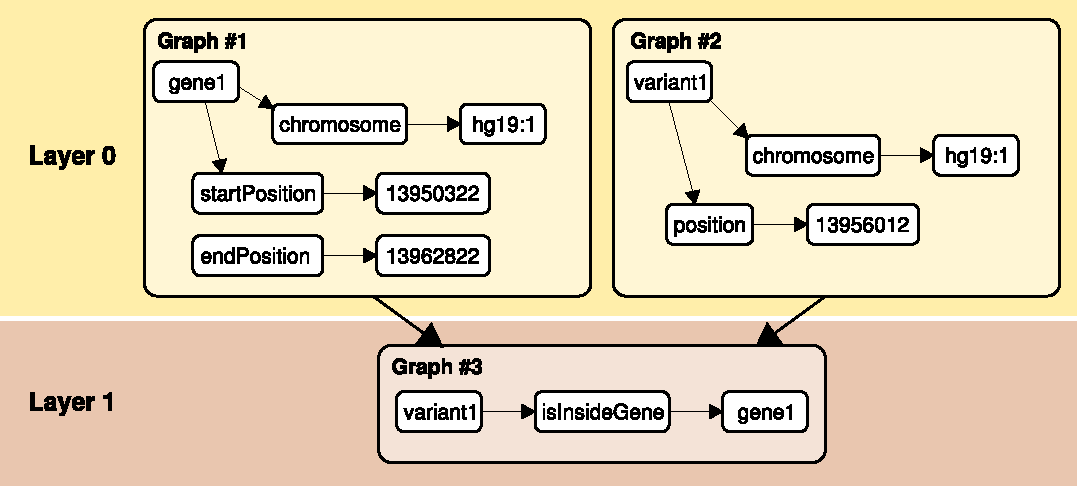
\includegraphics[width=1.0\textwidth]{figures/layered-knowledge.pdf}
    \end{center}
    \caption{\textit{An illustration of knowledge layers.}}
    \label{fig:layered-knowledge}
  \end{figure}

  Separating layers in graphs makes describing the flow of information easier,
  because the knowledge from a layer 1 graph can oftentimes be summarized as a
  query that described the relationship between the layer 0 graph(s) and the
  newly created layer 1 graph.

  Programs can operate on multiple layers of knowledge.  A program operates
  on the first layer (layer 0) when it translates a non-RDF format into RDF.
  These programs (re)state observations.  In the second layer (layer 1) and
  up, we find programs that operate on facts from layer 0 and generate
  inferences.

  From a computational perspective, these inferences allow programs to take
  shortcuts, and therefore answer questions (called \emph{querying}) faster.
  The performance of querying the graph can therefore be tuned by cleverly
  stating facts.  For example, by using the inference drawn in figure
  \ref{fig:layered-knowledge}, a query asking for ``all variants in a gene''
  no longer needs to compute whether a variant is inside any of the
  genes.  The query planner can also narrow the search space by only
  considering the variants in the layer 1 graph.

  From a data access perspective, these inferences allow fine-grained access
  to knowledge.  For example, access to a layer 1 graph can be given, but
  not to its underlying layer 0 graph(s).  Properties can be removed (like
  patient identifiers), or made less precise (only tell that there is a
  variant in a particular gene, rather than the variant details).

  The knowledge graph contains two types of nodes; uniquely identifiable
  names having a symbolic value (1), and literal values like numbers and
  text (2).  Nodes with a symbolic value, or simply \emph{symbols} can be used
  to add context to.  For example, consider the following statement:
  \triplet{<H>}{<electronegativity}{2.20}.  We can extend our knowledge
  about \code{<H>} by also stating: \triplet{<H>}{<numberOfElectrons>}{1}.
  The identifier \texttt{<H>} by itself has no meaning.  But that there is one
  ``thing'' for which both properties \texttt{<electronegativity>} and
  \texttt{<numberOfElectrons>} have a certain value provides insight into a
  deeper structure.

  We could go on and find more entities for which the properties
  \texttt{<electronegativity>} and \texttt{<numberOfElectrons>} are bound to
  specific values.  We can then identify the group of entities by a single
  \emph{type} to make it easier to talk about.   In the example, the type
  \texttt{<ChemicalElement>} may be suitable.  So we would add the triplet:
  \triplet{<H>}{rdf:type}{<ChemicalElement>}.

\section{Patterns for layer 0}

  The programs that are part of SPARQLing genomics use a few patterns to
  come up with identifiers.  For starters, the MD5 algorithm is used to come
  up with identifiers for the files that form the basis for layer 0.  We use
  a special URI prefix for these ``origins'':

  \ \ \ \ \triplet{<origin://d41d8cd98f00b204e9800998ecf8427e>}{rdf:type}
  {sg:Origin}

  By using a hashing algorithm we can safely assume that the identifiers will
  be the same when the input data was the same, regardless of who, when and
  in what order data was processed to (re)build the knowledge graph.

  This patterns is implemented by all programs described in chapter
  \refer{chap:command-line}.

\subsection{Public URIs and ontologies}
\label{sec:public-uris-and-ontologies}
  We have been using two types of symbols so far: internal (1) and publicly
  accessible (2).  We use the former for data-specific identifiers (like the
  MD5 sum for an origin) and the latter for increasing interoperability between
  distinct knowledge graphs.

  Such publicly accessible symbols are distributed in the form of a
  \emph{vocabulary} or \emph{ontology}.  In this manual the words ``vocabulary''
  and ``ontology'' are used interchangeably.  The use of symbols from various
  ontologies is the subject of chapter \refer{chap:implemented-ontologies}.


\ifdefined\HCode
\begin{html}
</div></div><div class="chapter"><div class="chapwrap">
\end{html}
\fi

\chapter{Use of ontologies}
\label{chap:implemented-ontologies}

  In chapter \refer{chap:knowledge-graph} we described publicly accessible
  symbols as the building blocks for ontologies.  In this chapter, we explain
  which ontologies we use, and how we use them.

  The following lookup table provides the name to abbreviate an ontology,
  and the full ontology URI.

  \hypersetup{urlcolor=black}
  \begin{table}[H]
    \begin{tabularx}{\textwidth}{*{1}{!{\VRule[-1pt]}l}!{\VRule[-1pt]}X}
      \headrow
      \textbf{Abbreviation} & \textbf{Ontology URI}\\
      \evenrow
      \texttt{dcterms} &
      \href{http://purl.org/dc/terms/}
           {http://purl.org/dc/terms/}\\
      \oddrow
      \texttt{dc} &
      \href{http://purl.org/dc/elements}{http://purl.org/dc/elements}\\
      \evenrow
      \texttt{faldo} &
      \href{http://biohackathon.org/resource/faldo\#}
      {http://biohackathon.org/resource/faldo\#}\\
      \oddrow
      \texttt{pato} &
      \href{http://purl.obolibrary.org/obo/}
           {http://purl.obolibrary.org/obo/}\\
      \evenrow
      \texttt{prov} &
      \href{http://www.w3.org/ns/prov\#}
           {http://www.w3.org/ns/prov\#}\\
      \oddrow
      \texttt{sg} &
      https://www.sparqling-genomics.org/\sgversion{}/\\
    \end{tabularx}
    \caption{\small Lookup table for ontology URIs and their abbreviations.}
    \label{table:ontology-abbreviations}
  \end{table}
  \hypersetup{urlcolor=LinkGray}

  In addition to these ontologies, we use the following internal prefixes in
  the remainder of the document.

  \hypersetup{urlcolor=black}
  \begin{table}[H]
    \begin{tabularx}{\textwidth}{*{1}{!{\VRule[-1pt]}l}!{\VRule[-1pt]}X}
      \headrow
      \textbf{Abbreviation} & \textbf{Ontology URI}\\
      \evenrow
      \texttt{bam2rdf} & \texttt{sg://\sgversion{}/bam2rdf/}\\
      \oddrow
      \texttt{table2rdf} & \texttt{sg://\sgversion{}/table2rdf/}\\
      \evenrow
      \texttt{json2rdf} & \texttt{sg://\sgversion{}/json2rdf/}\\
      \oddrow
      \texttt{vcf2rdf} & \texttt{sg://\sgversion{}/vcf2rdf/}\\
      \evenrow
      \texttt{xml2rdf} & \texttt{sg://\sgversion{}/xml2rdf/}\\
    \end{tabularx}
    \caption{\small Internal abbreviations used in the manual.}
    \label{table:internal-abbreviations}
  \end{table}
  \hypersetup{urlcolor=LinkGray}

\section{Describing genomic positions with FALDO}

  When describing the position of a nucleotide relative to its reference
  genome, we use the Feature Annotation Location Description Ontology (FALDO)
  \citep{Bolleman2016}. Table \ref{table:faldo-usage} provides an overview of
  the properties we use.

  \hypersetup{urlcolor=black}
  \begin{table}[H]
    \begin{tabularx}{\textwidth}{*{2}{!{\VRule[-1pt]}l}!{\VRule[-1pt]}X}
      \headrow
      \textbf{Term}     & \textbf{Used as} & \textbf{Usage}\\
      \evenrow
      \faldo{position}  & Predicate        & Used by \program{vcf2rdf} to
                                             describe the basepair position
                                             within a chromosome or contig.\\
      \oddrow
      \faldo{reference} & Predicate        & Used by \program{vcf2rdf} to
                                             describe the chromosome or contig
                                             to which the \faldo{position} is
                                             relative to.\\
    \end{tabularx}
    \caption{\small Terms used from FALDO.}
    \label{table:faldo-usage}
  \end{table}
  \hypersetup{urlcolor=LinkGray}

\section{Dublin Core Terms}

  In our published datasets and the \program{sg-web} interface, we use the Dublin
  Core Terms ontology \citep{dcmi-terms} to define organizations, collections,
  datasets, and samples.  Table \ref{table:dcterms-usage} provides an overview of
  the properties we use.

  \hypersetup{urlcolor=black}
  \begin{table}[H]
    \begin{tabularx}{\textwidth}{*{2}{!{\VRule[-1pt]}l}!{\VRule[-1pt]}X}
      \headrow
      \textbf{Term}   & \textbf{Used as} & \textbf{Description}\\
      \evenrow
      \dcterms{Agent}       & Object     & Used by \texttt{sg-web} to describe
                                           the user or organization that
                                           produced a collection or dataset.\\
      \oddrow
      \dctype{Collection}   & Object     & Reserved for a portal page in the web
                                           interface as a filter mechanism to
                                           browse \dctype{Dataset}s.\\
      \evenrow
      \dctype{Dataset}      & Object     & Reserved for a portal page in the web
                                           interface to describe data in a
                                           graph.\\
      \oddrow
      \dcterms{date}        & Object     & Used by \program{sg-web} to describe
                                           the time a query was run.\\
      \evenrow
      \dcterms{isPartOf}    & Predicate  & Reserved for a portal page in the web
                                           interface to express that a
                                           \dctype{Dataset} is linked to a
                                           \dctype{Collection}.\\
      \oddrow
      \dcterms{title}       & Predicate  & Used by \program{sg-web} to name a
                                           \dctype{Collection} or a
                                           \dctype{Dataset}.\\
      \evenrow
      \dcterms{publisher}   & Predicate  & Used by \program{sg-web} to identify
                                           the organization that published
                                           a collection or dataset.\\
      \oddrow
      \dcterms{description} & Predicate  & Used by \program{sg-web} to provide
                                           a textual description of a
                                           \dctype{Collection} or a
                                           \dctype{Dataset}.\\
    \end{tabularx}
    \caption{\small Terms used from the Dublic Core Terms ontology.}
    \label{table:dcterms-usage}
  \end{table}
  \hypersetup{urlcolor=LinkGray}

\section{Provenance tracking with PROV-O}

  To maintain an understanding of ``who did what?'' when it comes to importing,
  modifying, removing, and querying data in the knowledge graph, we use parts of
  the PROV ontology \citep{prov-o}.

  \hypersetup{urlcolor=black}
  \begin{table}[H]
    \begin{tabularx}{\textwidth}{*{2}{!{\VRule[-1pt]}l}!{\VRule[-1pt]}X}
      \headrow
      \textbf{Term}        & \textbf{Used as} & \textbf{Usage}\\
      \evenrow
      \prov{startedAtTime} & Predicate        & Used by \program{sg-web} to
                                                describe the date and time a
                                                query was run.\\
      \oddrow
      \prov{endedAtTime}   & Predicate        & Used by \program{sg-web} to
                                                describe the date and time a
                                                query finished.\\
    \end{tabularx}
    \caption{\small Terms used from PROV-O.}
    \label{table:prov-usage}
  \end{table}
  \hypersetup{urlcolor=LinkGray}

\section{Phenotype And Trait Ontology}

  When describing phenotype properties, we use the Phenotype And Trait
  Ontology (PATO) \citep{pato}.  Table \ref{table:pato-usage} provides an
  overview of the properties we use.

  \hypersetup{urlcolor=black}
  \begin{table}[H]
    \begin{tabularx}{\textwidth}{*{2}{!{\VRule[-1pt]}l}!{\VRule[-1pt]}X}
      \headrow
      \textbf{Term}       & \textbf{Used as} & \textbf{Usage}\\
      \evenrow
      \obo{PATO\_0000384} & Object           & Used in the published datasets
                                               to describe a donor as male.\\
      \oddrow
      \obo{PATO\_0000383} & Object           & Used in the published datasets
                                               to describe a donor as female.\\
      \evenrow
      \obo{PATO\_0001894} & Predicate        & Used in the published datasets
                                               to describe the phenotypic sex.\\
    \end{tabularx}
    \caption{\small Terms used from PATO.}
    \label{table:pato-usage}
  \end{table}
  \hypersetup{urlcolor=LinkGray}

\section{Custom terms}

  Sometimes we miss the right term to describe a statement.  In such cases we
  decide on a new term that is then part of the \emph{SPARQLing-genomics
    ontology}.  The use of these terms is subject to change in upcoming versions
  of \texttt{sparqling-genomics}.  Table \ref{table:sg-usage} summarizes the
  terms that are waiting to be replaced by an external ontology.

  \hypersetup{urlcolor=black}
  \begin{table}[H]
    \begin{tabularx}{\textwidth}{*{2}{!{\VRule[-1pt]}l}!{\VRule[-1pt]}X}
      \headrow
      \textbf{Term} & \textbf{Used as} & \textbf{Usage}\\
      \evenrow
      \sg{Origin}   & Object           & Used by the command-line tools (see
                                         chapter \refer{chap:command-line})
                                         to point to the file or resource from
                                         which information was derived.\\
      \oddrow
      \sg{Sample}   & Object           & Used by \program{vcf2rdf} and
                                         \program{bam2rdf} to describe a
                                         sample.\\
    \end{tabularx}
    \caption{\small Custom terms used by SPARQLing-genomics.}
    \label{table:sg-usage}
  \end{table}
  \hypersetup{urlcolor=LinkGray}


\ifdefined\HCode
\begin{html}
</div></div><div class="chapter"><div class="chapwrap">
\end{html}
\fi

\chapter{Command-line programs}
\label{chap:command-line}

  SPARQLing genomics provides programs to create an extensive knowledge graph
  from various domain-specific data formats.  The programs described in this
  chapter provide the ``layer 0'' for the knowledge graph, and the tools to
  discover the data in this layer.   All tools described in the remainder of
  this chapter can be invoked with the \t{-{}-help} argument to get a
  complete overview of options for that particular tool.

\section{Preparing variant call data with \program{vcf2rdf}}
\label{sec:vcf2rdf}

  Variant callers extract variation from sequenced data.  These programs
  often output the variants they found in the \i{Variant Call Format}
  (VCF) or its binary equivalent (BCF).  The \program{vcf2rdf} program
  extracts knowledge from a VCF or BCF file and writes it as RDF.

\subsection{Knowledge extracted by \program{vcf2rdf}}

  The program treats the VCF as its own ontology.  It uses the VCF header as
  a guide.  All fields described in the header of the VCF file will be
  translated into triples.  In addition to the knowledge from the VCF file,
  \program{vcf2rdf} provides the following triples:

  \begin{table}[H]
    \begin{tabularx}{\textwidth}{*{3}{!{\VRule[-1pt]}l}!{\VRule[-1pt]}L}
      \headrow
      \b{Subject}       & \b{Predicate}    & \b{Object}
      & \b{Description}\\
      \evenrow
      \origin{\i{MD5}}  & \rdf{type}       & \sg{Origin}
      & This defines a uniquely identifiable reference to the originating file.\\
      \oddrow
      \origin{\i{MD5}}  & \sg{filename}    & \i{filename}
      & This triple states the originating filename.\\
      \evenrow
      \origin{\i{MD5}}  & \sg{md5}         & \i{MD5 sum}
      & This triple states the MD5 sum of the content of the original file.\\
      \oddrow
      \sample{\i{name}} & \rdf{type}       & \sg{Sample}
      & This states that there is a sample with \i{sample name}.\\
      \evenrow
      \sample{\i{name}} & \sg{foundIn}     & \origin{\i{MD5}}
      & This triple states that a sample can be found in a file identified by
      the \sg{Origin} with a specific identifier.\\
      \oddrow
      \origin{\i{MD5}}  & \sg{convertedBy} & \sgv{vcf2rdf}
      & This triple states that the file was converted with \program{vcf2rdf}.\\
    \end{tabularx}
    \caption{\small The additional triple patterns provided by \program{vcf2rdf}.}
    \label{table:vcf2rdf-ontology}
  \end{table}

  The following snippet is an example of the extra data in Turtle-format:

\begin{lstlisting}
@prefix sg: <https://sparqling-genomics.org/(@*\sgversion{}*@)/> .
@prefix orig: <origin://> .

orig:e9e38f2e4279eda346918ba69fd86c5f
    a sg:Origin ;
    sg:convertedBy <https://sparqling-genomics.org/(@*\sgversion{}*@)/vcf2rdf-(@*\sgversion{}*@)> ;
    sg:filename "tests/sample.vcf"^^xsd:string ;
    sg:md5 "e9e38f2e4279eda346918ba69fd86c5f"^^xsd:string .

<origin://e9e38f2e4279eda346918ba69fd86c5f@S0>
    a sg:Sample ;
    rdfs:label "SAMLPEA"^^xsd:string ;
    sg:foundIn orig:e9e38f2e4279eda346918ba69fd86c5f .
\end{lstlisting}

\subsection{Handling multi-sample VCF files}

  From version \t{0.99.11} onwards, \program{vcf2rdf} only writes variants
  that have at least one alternative allele specified.  It will reserve the
  numeric ID to preserve compatibility with previous and future versions.

  The numeric IDs are calculated left-to-right, top-to-bottom.  So for a file
  containing two samples, the first variant for the first sample will receive
  the numeric ID $0$, and the first variant for the second sample will receive
  numeric ID $1$.  The second variant for the first sample receives numeric ID
  $2$, and so on.

\subsection{Example usage}

The following command invocation will produce RDF in the \t{ntriples}
format:

\begin{lstlisting}
vcf2rdf -i /path/to/my/variants.vcf > /path/to/my/variants.n3
\end{lstlisting}

To get a complete overview of options for this program, use:

\begin{lstlisting}
vcf2rdf --help
\end{lstlisting}

\subsection{Run-time properties}

  Depending on the serialization format, the program typically uses from two megabytes
  (in \t{ntriples} mode), to multiple times the size of the input VCF
  (in \t{turtle} mode).

  The \t{ntriples} mode can output triples as soon as they are formed, while the
  \t{turtle} mode waits until all triples are known, so that it can output them
  efficiently, producing compact output at the cost of using more memory.

  We recommend using the \t{ntriples} format for large input files, and
  \t{turtle} for small input files.  The following example illustrates how to
  use \t{turtle} mode.

\begin{lstlisting}
vcf2rdf -i /path/to/my/variants.vcf -O turtle > /path/to/my/variants.ttl
\end{lstlisting}

\section{Preparing sequence alignment maps with \program{bam2rdf}}

  When DNA sequencing reads are aligned to a predetermined \i{reference
  genome}, it's often formatted in the \i{sequence alignment map} (SAM)
  format, its equivalent \i{binary alignment map} (BAM) format, or its
  equivalent CRAM format.  The \program{bam2rdf} program can read data in all
  three formats.

\subsection{Knowledge extracted by \program{bam2rdf}}

  The current version of \program{bam2rdf} merely extracts information from the
  alignment map header.  In addition to the knowledge from the file, it also
  produces the following metadata:

  \begin{table}[H]
    \begin{tabularx}{\linewidth}{>{\hsize=0.18\hsize}X
        !{\VRule[-1pt]}>{\hsize=0.20\hsize}X
        !{\VRule[-1pt]}>{\hsize=0.32\hsize}L
        !{\VRule[-1pt]}>{\hsize=0.30\hsize}L}
      \headrow
      \b{Subject}      & \b{Predicate} & \b{Object}
      & \b{Description}\\
      \evenrow
      \origin{\i{MD5}} & \rdf{type}    & \sg{Origin}
      & This defines a uniquely identifiable reference to the originating file.\\
      \oddrow
      \origin{\i{MD5}} & \sg{filename} &  \i{filename}
      & This triple states the originating filename.\\
      \evenrow
      \origin{\i{MD5}} & \rdf{type}    & One of: \bamrdf{HeaderItem},
      \bamrdf{ReferenceSequence}, \bamrdf{ReadGroup}, \bamrdf{Program},
      \bamrdf{Comment}.
      & The \i{objects} correspond to the various types of header lines that
      can occur in the SAM format.\\
      \oddrow
      \origin{\i{MD5}} & \bamrdf{\i{type}/\i{key}} & Literal value.
      & Each header field consists of a key/value pair.  The key is used as
      predicate.\\
      \oddrow
      \origin{\i{MD5}} & \sg{convertedBy} & \sgv{bam2rdf}
      & This triple states that the file was converted with \program{bam2rdf}.\\
    \end{tabularx}
    \caption{\small The additional triple patterns provided by \program{bam2rdf}.}
    \label{table:bam2rdf-ontology}
  \end{table}

\subsection{Example usage}

The following command invocation will produce RDF in the \t{ntriples}
format:

\begin{lstlisting}
bam2rdf -i /path/to/my/sequencing_data.bam > /path/to/my/sequencing_data.n3
\end{lstlisting}

To get a complete overview of options for this program, use:

\begin{lstlisting}
bam2rdf --help
\end{lstlisting}

\section{Preparing tabular data with \program{table2rdf}}
\label{sec:table2rdf}

  Data that can be represented as a table, like comma-separated values (CSV)
  or BED files, can be imported using \program{table2rdf}.  The column headers
  are used as predicates, and each row gets a unique row ID.  Non-alphanumeric
  characters in the header line are replaced by underscores, and all characters
  are replaced by their lowercase equivalent to make a consistent scheme for
  predicates.

  When the file does not contain a header line, one can be specified using the
  \t{-{}-header-line} argument.  When using this command-line argument, the
  delimiter must be a semicolon (\t{;}).

  The program can also read files compressed with \program{gzip}.

\subsection{Transforming objects}

  Unfortunately, \program{table2rdf} knows nothing about ontologies.  So when
  the input table has a column ``Chromosome'', by default \program{table2rdf}
  will treat these cells as literal values (as a \t{string}).  A
  \i{transformer} can be used to express a column as an \i{individual} in
  RDF.  An example might explain this best.

  Take the following input file:

\begin{lstlisting}
$ cat test.tsv
Chromosome      Position
chr1    1500000
chrMT   11000
\end{lstlisting}

  Running \program{table2rdf} with its default settings will produce:

\begin{lstlisting}
$ table2rdf -i test.tsv -O turtle
...
<origin://...@0>
    sg:originatedFrom <http://sparqling-genomics/...> ;
    col:chromosome "chr1"^^xsd:string ;
    col:position 1500000 ;
    a :Row .

<origin://...@1>
    sg:originatedFrom <http://sparqling-genomics/...> ;
    col:chromosome "chrMT"^^xsd:string ;
    col:position 11000 ;
    a :Row .
...
\end{lstlisting}

  \begin{sloppypar}
  When we know that the data in a column refers to items in an ontology, like
  chromosomes defined in
  \href{http://rdf.biosemantics.org/data/genomeassemblies/hg19}%
  {<http://rdf.biosemantics.org/data/genomeassemblies/hg19>}, \program{table2rdf}
  can be told to use that ontology to describe that column.
  \end{sloppypar}

  To do so, we use the \t{-{}-transform-object} option, or \t{-t}
  for short:

\begin{lstlisting}
$ table2rdf -O turtle \
    -i test.tsv       \
    -t Chromosome=http://rdf.biosemantics.org/data/genomeassemblies/hg19#
...
(@*\colorbox{Highlight}{@prefix p00000: <http://rdf.biosemantics.org/data/genomeassemblies/hg19\#> .}*@)
...
<http://sparqling-genomics/table2rdf/Row/...-R0000000000>
    sg:originatedFrom <http://sparqling-genomics/...> ;
    (@*\colorbox{Highlight}{col:chromosome p00000:chr1 ;}*@)
    col:position 1500000 ;
    a :Row .

<http://sparqling-genomics/table2rdf/Row/...-R0000000001>
    sg:originatedFrom <http://sparqling-genomics/...> ;
    (@*\colorbox{Highlight}{col:chromosome p00000:chrMT ;}*@)
    col:position 11000 ;
    a :Row .
...
\end{lstlisting}

  After the transformation, the output produced by \t{table2rdf} uses
  URIs pointing to the ontology instead of literal values for chromosomes.

\subsection{Transforming predicates}

  Like transforming a cell in a table to a URI instead of a literal value,
  we can also specify the value for the column name.  By default, the column
  names are transformed using the \tablerdf{Column/} prefix (e.g.
  \t{chromosome} becomes
  \t{sg://\sgversion{}/table2rdf/Column/chromosome}).  By using
  the \t{-{}-transform-predicate} option, or \t{-T} for short, a
  different transformation can be made:

\begin{lstlisting}
$ table2rdf -O turtle \
    -i test.tsv       \
    -t Chromosome=http://rdf.biosemantics.org/data/genomeassemblies/hg19# \
    -T Chromosome=http://biohackathon.org/resource/faldo#reference
...
(@*\colorbox{Highlight}{@prefix p00000: <http://rdf.biosemantics.org/data/genomeassemblies/hg19\#> .}*@)
(@*\colorbox{Highlight}{@prefix p00001: <http://biohackathon.org/resource/faldo\#> .}*@)

<origin://...@0>
    sg:originatedFrom <origin://...> ;
    (@*\colorbox{Highlight}{p00001:reference p00000:chr1 ;}*@)
    col:position 1500000 ;
    a :Row .

<origin://...@1>
    sg:originatedFrom <origin://...> ;
    (@*\colorbox{Highlight}{p00001:reference p00000:chrMT ;}*@)
    col:position 11000 ;
    a :Row .
...
\end{lstlisting}

\subsection{Delimiters}

  Tabular data consists of rows and columns.  A field is a specific place in
  a table, having a column-coordinate, and a row-coordinate.  To distinguish
  fields from one another we use a delimiter.  Which delimiter to use (a tab,
  a comma, or a semicolon, etc.) is up to the dataset.  The delimiter
  can be chosen using the \t{-{}-delimiter} option, or \t{-d} for
  short.

  Sometimes a single field can consist of multiple ``subfields''.  To
  distinguish subfields, we use a secondary delimiter.  In RDF, we can split
  those subfields by using the same predicate as we would use for the entire
  field.  Using the \t{-{}-secondary-delimiter} option, we can invoke
  this behavior.

  The following example demonstrates the usage of \t{-{}-delimiter} and
  \t{-{}-secondary-delimiter}.  Take the following input file:

\begin{lstlisting}
$ cat multi.tsv
Chromosome	Position	Filter
1	10000	A;B;C;D
\end{lstlisting}

  Without using the secondary delimiter, we get:

\begin{lstlisting}
$ table2rdf -i multi.tsv -O turtle
...
<origin://...@0>
    sg:originatedFrom <http://sparqling-genomics/...> ;
    col:chromosome 1 ;
    (@*\colorbox{Highlight}{col:filter "A;B;C;D"\^{}\^{}xsd:string ;}*@)
    col:position 10000 ;
    a :Row .
\end{lstlisting}

  Using the secondary delimiter, we get:

\begin{lstlisting}
$ table2rdf -i multi.tsv --secondary-delimiter ";" -O turtle
...
<origin://...@0>
    sg:originatedFrom <http://sparqling-genomics/...> ;
    col:chromosome 1 ;
    (@*\colorbox{Highlight}{col:filter "A"\^{}\^{}xsd:string, "B"\^{}\^{}xsd:string, "C"\^{}\^{}xsd:string,}*@)
    (@*\colorbox{Highlight}{\space\space\space\space\space\space\space\space\space\space\space"D"\^{}\^{}xsd:string ;}*@)
    col:position 10000 ;
    a :Row .
\end{lstlisting}

  Notice how the \t{col:filter} predicate now describes a
  connection to four objects instead of one.

\subsection{Knowledge extracted by \program{table2rdf}}

  The \program{table2rdf} program extracts all fields in the table.  In addition
  to the knowledge from the table file, \program{table2rdf} stores the following
  metadata:

    \begin{table}[H]
      \begin{tabularx}{\textwidth}{*{3}{!{\VRule[-1pt]}l}!{\VRule[-1pt]}L}
      \headrow
      \b{Subject}     & \b{Predicate}    & \b{Object}
      & \b{Description}\\
      \evenrow
      \origin{\i{MD5}}  & \rdf{type}            & \sg{Origin}
      & This defines a uniquely identifiable reference to the originating
        file.\\
      \oddrow
      \origin{\i{MD5}}  & \t{:filename}    & \i{filename}
      & This triple states the originating filename.\\
      \evenrow
      \origin{\i{MD5}}  & \t{:convertedBy} & \sgv{table2rdf}
      & This triple states that the file was converted with
        \program{table2rdf}.\\
    \end{tabularx}
    \caption{\small The additional triple patterns provided by \program{table2rdf}.}
    \label{table:table2rdf-ontology}
  \end{table}

  The following snippet is an example of the extra data in Turtle-format:

\begin{lstlisting}
<origin://1jka8923i4>
    :convertedBy :table2rdf ;
    :filename "grch37.bed"^^xsd:string ;
    a :Origin .

sample:grch37
    :foundIn <origin://1jka8923i4> ;
    a :Sample .
\end{lstlisting}

\subsection{Example usage}

The following command invocation will produce RDF in the \t{ntriples}
format:

\begin{lstlisting}
table2rdf -i /path/to/my/table.tsv > /path/to/my/table.n3
\end{lstlisting}

To get a complete overview of options for this program, use:

\begin{lstlisting}
table2rdf --help
\end{lstlisting}

\section{Converting MySQL data to RDF with \program{table2rdf}}

  Relational databases store data in tables.  With \program{table2rdf} we
  can oftentimes convert the data in a single go to RDF triples.  The following
  example extracts the \t{regions} table from a MySQL server in a database
  called \t{example}.

\begin{lstlisting}
mysql --host=127.0.0.1 -e "SELECT * FROM example.regions" \
      --batch | table2rdf --stdin > regions.n3
\end{lstlisting}

  The \program{mysql} command outputs the table in tab-delimited form when using
  the \t{-{}-batch} argument, which is the default input type for
  \program{table2rdf}.  To accept input from a UNIX pipe \program{table2rdf} must
  be invoked with the \t{-{}-stdin} argument.

\section{Preparing XML data with \program{xml2rdf}}
\label{sec:xml2rdf}

  Data encoded in the EXtensible Markup Language (XML) can be converted to RDF
  in a naive way by \program{xml2rdf}.  A child element refers to its parent with
  the \sg{isPartOf} predicate.

  \begin{table}[H]
    \begin{tabularx}{\textwidth}{*{3}{!{\VRule[-1pt]}l}!{\VRule[-1pt]}L}
      \headrow
      \b{Subject}    & \b{Predicate}    & \b{Object}
      & \b{Description}\\
      \evenrow
      \origin{\i{MD5}} & \rdf{type}            & \sg{Origin}
      & This defines a uniquely identifiable reference to the originating
        file.\\
      \oddrow
      \origin{\i{MD5}} & \sg{filename}         & \i{filename}
      & This triple states the originating filename.\\
      \evenrow
      \origin{\i{MD5}} & \sg{convertedBy}      & \sgv{xml2rdf}
      & This triple states that the file was converted with
        \program{xml2rdf}.\\
    \end{tabularx}
    \caption{\small The triplet patterns used by \program{xml2rdf}.}
    \label{table:xml2rdf-ontology}
  \end{table}

\subsection{Example usage}
The following command invocation will produce RDF in the \t{ntriples}
format:

\begin{lstlisting}
xml2rdf -i /path/to/my/data.xml > /path/to/my/data.n3
\end{lstlisting}

To get a complete overview of options for this program, use:

\begin{lstlisting}
xml2rdf --help
\end{lstlisting}

\section{Preparing JSON data with \program{json2rdf}}
\label{sec:json2rdf}

  The JavaScript Object Notation (JSON) has become a popular format
  for encoding information from and to web APIs.  With \program{json2rdf},
  a layer 0 representation in RDF can be created.

\subsection{Knowledge extracted by \program{json2rdf}}

  Each key-value pair is translated into \triplet{Unique ID}{key}{value}.
  When the value of a pair contains a structure with more key-value pairs,
  the triplet's value refers to the \t{unique-id} assigned to that
  structure.  In addition to the key-value pairs, \program{json2rdf} stores
  the following metadata:

  \begin{table}[H]
    \begin{tabularx}{\textwidth}{*{3}{!{\VRule[-1pt]}l}!{\VRule[-1pt]}L}
      \headrow
      \b{Subject} & \b{Predicate} & \b{Object}
      & \b{Description}\\
      \evenrow
      \origin{\i{MD5}}  & \rdf{type}       & \sg{Origin}
      & This defines a uniquely identifiable reference to the originating file.\\
      \oddrow
      \origin{\i{MD5}}  & \sg{filename}    & \i{filename}
      & This triple states the originating filename.\\
      \evenrow
      \origin{\i{MD5}} & \sg{convertedBy}  & \sgv{json2rdf}
      & This triple states that the file was converted with
        \program{json2rdf}.\\
    \end{tabularx}
    \caption{\small The triplet patterns used by \program{xml2rdf}.}
    \label{table:json2rdf-ontology}
  \end{table}

\subsection{Example usage}

The following command invocation will produce RDF in the \t{ntriples}
format:

\begin{lstlisting}
json2rdf -i /path/to/my/data.json > /path/to/my/data.n3
\end{lstlisting}

To get a complete overview of options for this program, use:

\begin{lstlisting}
json2rdf --help
\end{lstlisting}

\section{Extracting knowledge from folders with \t{folder2rdf}}
\label{sec:folder2rdf}

  The \program{folder2rdf} program finds files in a directory to extract
  knowledge from.  It attempts to convert files with extensions
  \t{.vcf}, \t{.vcf.gz}, \t{.bcf}, and \t{.bcf.gz}
  using \program{vcf2rdf}, and files with extensions \t{.sam},
  \t{.bam}, and \t{.cram} using \program{bam2rdf}.

\subsection{Example usage}

\begin{lstlisting}
folder2rdf --input-directory=/vcf-data   \
           --output-directory=/rdf-data  \
           --project-name Example        \
           --recursive                   \
           --compress                    \
           --threads=4
\end{lstlisting}

  $\ldots{}$ where \t{/vcf-data} is a directory containing VCF files,
  and \t{/rdf-data} is the directory to store the converted files.

\subsection{Knowledge extracted by \program{folder2rdf}}

  In addition to the knowledge extracted by \program{vcf2rdf}, this program
  extracts the following data:

  \begin{table}[H]
    \begin{tabularx}{\textwidth}{*{3}{!{\VRule[-1pt]}l}!{\VRule[-1pt]}L}
      \headrow
      \b{Subject}                 & \b{Predicate} & \b{Object}
      & \b{Description}\\
      \evenrow
      \project{\i{project-name}}    & \rdf{type}         & \sg{Project}
      & This defines the identifier for the project.\\
      \oddrow
      \user{\i{username}}           & \rdf{type}         & \sg{User}
      & This defines the identifier for the file owner (username).\\
      \evenrow
      \origin{\i{MD5}}              & \rdf{type}         & \sg{Origin}
      & This defines a uniquely identifiable reference to the originating
      file.\\
    \end{tabularx}
    \caption{\small The additional triple patterns produced by \program{folder2rdf}.}
    \label{table:folder2rdf-ontology}
  \end{table}

\section{Importing data with \program{curl}}
\label{sec:curl}

  To load RDF data into a triple store (our database), we can use \program{curl}.

  The triple stores typically store data in \i{graphs}.  One triple store
  can host multiple graphs, so we must tell the triple store which graph we
  would like to add the data to.

\subsection{Example usage}

% Other types: application/n-triples

\begin{lstlisting}
curl -X POST                                                 \
     -H "Content-Type: text/turtle"                          \
     -T /path/to/variants.ttl                                \
     -G <endpoint URL>                                       \
     --digest -u <username>:<password>                       \
     --data-urlencode graph=http://example/graph
\end{lstlisting}

\subsubsection{Virtuoso example}

\begin{sloppypar}
The following example inserts the file \t{vcf2rdf-variants.ttl} into
a graph called \t{http://example/graph} in a Virtuoso endpoint at
\url{http://127.0.0.1:8890} with the username \t{dba} and
password \t{qwerty}.
\end{sloppypar}

\begin{lstlisting}
curl -X POST                                                 \
     -H "Content-Type: text/turtle"                          \
     -T vcf2rdf-variants.ttl                                 \
     -G http://127.0.0.1:8890/sparql-graph-crud-auth         \
     --digest -u dba:qwerty                                  \
     --data-urlencode graph=http://example/graph
\end{lstlisting}

\subsubsection{4store example}

Similar to the Virtuoso example, for \program{4store} the command looks like
this:

\begin{lstlisting}
curl -X POST                                                 \
     -H "Content-Type: text/turtle"                          \
     -T vcf2rdf-variants.ttl                                 \
     -G http://127.0.0.1:8080/data/http://example/graph
\end{lstlisting}

Notice that \program{4store} does not provide an authentication mechanism.

\subsubsection{Sending \t{gzip}-compressed data}

  When the RDF file is compressed with \program{gzip}, extra HTTP headers must
  be added to the \program{curl} command:

\begin{lstlisting}
curl -X POST                                                 \
     -H "Content-Type: text/turtle"                          \
     -H "Transfer-Encoding: chunked"                         \
     -H "Content-Encoding: gzip"                             \
     ...
\end{lstlisting}


\ifdefined\HCode
\begin{html}
</div></div><div class="chapter"><div class="chapwrap">
\end{html}
\fi

\chapter{Web interface}
\label{chap:web-interface}
\index{sg-web}

  The command-line programs described in chapter \refer{chap:command-line}
  provide data for layer \t{0}.  With the web interface described in
  this chapter, this data can be further structured, analyzed, and shared.
  In short, with the web interface you can:
  \begin{itemize}
  \item Manage data and data access across RDF stores;
  \item Write, execute, and share SPARQL queries;
  \item Explore the inner-structure of datasets.
  \end{itemize}

\section{Setting up the web interface}
\label{sec:configuring-sg-web}

  Before the web interface can be started, a few parameters have to be
  configured.  This is done through an XML file.  The following example
  displays all options, except for the authentication part, which is
  discussed separately in section \refer{sec:authentication}.

\begin{siderules}
\begin{verbatim}
<?xml version="1.0" encoding="utf-8"?>
<web-interface>
  <fork>0</fork>
  <bind-address>127.0.0.1</bind-address>
  <port>8080</port>
  <developer-mode>0</developer-mode>
  <backtrace-on-error>0</backstrace-on-error>
  <upload-root>/data</upload-root>
  <system-connection>
    <uri>http://localhost:8890/sparql-auth</uri>
    <backend>virtuoso</backend>
    <username>dba</username>
    <password>dba</password>
  </system-connection>
  <authentication>
    <!-- Either LDAP settings, or local-user authentication -->
  </authentication>
</web-interface>
\end{verbatim}
\end{siderules}

\subsection{To fork or not to fork}

  The \t{fork} property can be either \t{0} to keep the
  \program{sg-web} process in the foreground of your shell, or
  \t{1} to run the \program{sg-web} process as a daemon.

\subsection{Bind address and port}

  To enable running multiple web services on single machine, \program{sg-web}
  can be configured to bind on an arbitrary address and an arbitrary port.
  Both IPv4 and IPv6 addresses are supported.

\subsection{Developer mode}

  By default, changes to code in the \file{www/pages/} directory are
  applied when restarting \program{sg-web}.  When turning on
  `\t{developer-mode}', pages are reloaded when accessed, which makes
  interactive development of web pages easier.

\subsection{Logging and backtraces}
\label{sec:logging}

  The \program{sg-web} program keeps two logs: one for error reporting, and
  one for access and non-critical messages.  The log files can be specified
  as command-line options (\t{-e} for error reporting, \t{-d} for
  non-critical messages).

  Backtraces help the developer to get an idea about how something might've
  gone wrong.  It displays the location nearby the location in the source code
  that throwed an error.  Backstraces can get long and verbose.  Therefore we
  don't display them by default.  To enable reporting backtraces in the error
  log, set the `\t{backtrace-on-error}' option to \t{1}.

\subsection{Upload directory}

  Users can upload RDF files to import it into an RDF store.  The files must
  be stored on the filesystem.  With \t{upload-root}, the location of
  the upload directory can be changed.  It can also be set using the
  environment variable \t{SG\_WEB\_UPLOAD\_ROOT}.  If none of these are
  specified, the value of the environment variable \t{TMPDIR} will be
  used, or when that is not set, \file{/tmp} will be used.

\subsection{System connection}

  The web interface stores its own information as RDF.  Therefore it needs
  a connection to an RDF store where it can write to the graphs described
  in table \ref{table:writable-graphs}.

  \hypersetup{urlcolor=black}
  \begin{table}[H]
    \begin{tabularx}{\textwidth}{l!{\VRule[-1pt]}X}
      \headrow
      \b{Graph} & \b{Reason}\\
      \evenrow
      \t{http://sparqling-genomics.org/sg-web/state}
      & In this graph, queries and projects are stored.\\
    \end{tabularx}
    \caption{\small Graphs that need to be writable for the web interface.}
    \label{table:writable-graphs}
  \end{table}
  \hypersetup{urlcolor=LinkGray}

\subsubsection{System connection example}

  To configure the \i{system connection}, two parameters need to be
  specified: \t{uri}, and \t{backend}.  Additionally, when the
  RDF store requires authentication for writing to it, a \t{username}
  and a \t{password} can be provided.

  The following example shows how to configure the \i{system connection}:

\begin{siderules}
\begin{verbatim}
<?xml version="1.0" encoding="utf-8"?>
<web-interface>
  ...
  <system-connection>
    <uri>http://localhost:8890/sparql-auth</uri>
    <backend>virtuoso</backend>
    <username>dba</username>
    <password>dba</password>
  </system-connection>
</web-interface>
\end{verbatim}
\end{siderules}

\subsection{Beacon support}
\label{sec:beacon}

  Beacon is an interface to create a ``global search engine for genetic
  mutations'' \citep{beacon-network}.  It achieves this by defining a
  standard that institutions must implement so that one search engine can
  query the implementations from each institution to find a specific
  genetic mutation.

  The web interface can function as a Beacon in the Beacon network
  \citep{beacon-network}.  The Beacon API uses a separate connection,
  similar to the \t{system-connection}, so that access can be
  controlled at the user level.

  The following example shows how to configure \i{Beacon} including the
  \i{Beacon connection}:

\begin{siderules}
\begin{verbatim}
<?xml version="1.0" encoding="utf-8"?>
<web-interface>
  ...
  <beacon>
    <enabled>1</enabled>
    <organization>
      <id>SG</id>
      <name>SPARQLing-genomics Beacon service</name>
      <description>
        This Beacon service provides variant information for data hosted by
        this instance of the RDF store.
      </description>
      <address>Not provided</address>
      <welcome-url>https://www.sparqling-genomics.org</welcome-url>
      <contact-url>mailto:beacon@sparqling-genomics.org</contact-url>
      <logo-url>https://www.sparqling-genomics.org/static/images/logo.png</logo-url>
      <info>Not provided</info>
    </organization>
    <connection>
      <uri>http://localhost:8000</uri>
      <backend>virtuoso</backend>
      <username>beacon</username>
      <password>changeme</password>
    </connection>
  </beacon>
</web-interface>
\end{verbatim}
\end{siderules}

  The implementation assumes the following conditions are met:
  \begin{itemize}
  \item Variant call data was imported using \t{vcf2rdf};
  \item The reference genome can be identified by the chromosome's NCBI
    identifier.
  \end{itemize}

\subsection{User management and authentication}
\label{sec:authentication}

  The \program{sg-web} assumes every user of the system has a username
  and a password to authenticate oneself. There are two ways to configure
  authentication.  For isolated deployments or environments, preconfigured
  accounts can be specified.  For organizational deployments, the web interface
  can be configured to use an LDAP server that supports version 3 of the LDAP
  protocol.

  Regardless of the authentication mechanism, there are a few reserved users
  that carry out a specific task within \program{sg-web}.  The table below
  describes the reserved users.

  \hypersetup{urlcolor=black}
  \begin{table}[H]
    \begin{tabularx}{\textwidth}{l!{\VRule[-1pt]}X}
      \headrow
      \b{Username} & \b{Task}\\
      \evenrow
      \t{beacon}
      & When the BEACON API (see section \refer{sec:beacon}) is enabled, and
      this user is added to a project, the data that is accessible by the
      project will be exposed to the BEACON network.\\
      \oddrow
      \t{portal}
      & This username has been reserved for an implementation of a data
      portal.\\
    \end{tabularx}
    \caption{\small Reserved users for \program{sg-web}.}
    \label{table:reserved-users}
  \end{table}
  \hypersetup{urlcolor=LinkGray}

\subsubsection{Local users configuration}

  The simplest form of authentication is the ``local-user configuration''.
  Configuring it involves providing a username and the SHA256 sum of a password
  for each account.  The following example shows how to configure
  ``local-user authentication'':

\begin{siderules}
\begin{verbatim}
<?xml version="1.0" encoding="utf-8"?>
<web-interface>
  ...
  <authentication>
    <user>
      <username>user</username>
      <!-- The password field must contain the SHA256 sum of the
           plaintext password -->
      <password>9f86d08...0f00a08</password>
    </user>
    <user>
      <username>user2</username>
      <password>152f347...0b7a26a</password>
    </user>
  </authentication>
</web-interface>
\end{verbatim}
\end{siderules}

\subsubsection{LDAP authentication example}

  To configure LDAP, four parameters must be specified: the URI to the LDAP
  service (1), optionally, an extra ``common name'' (2), optionally the
  ``organizational unit'' (3), and the ``domain'' (4).  The username is used
  as a ``common name''.

  \begin{sloppypar}
  Additionally, an alternative SSL certificate bundle can be configured with
  the parameters \t{ssl-certificate-directory} and
  \t{ssl-certificate-file}.
  \end{sloppypar}

  The following example shows how to configure LDAP authentication:

\begin{siderules}
\begin{verbatim}
<?xml version="1.0" encoding="utf-8"?>
<web-interface>
  ...
  <authentication>
    <ldap>
      <uri>ldaps://example.local</uri>
      <common-name>AdditionalCN</common-name>
      <organizational-unit>People</organizational-unit>
      <domain>department.organization.tld</domain>
      <ssl-certificate-directory>/etc/ssl/certs</ssl-certificate-directory>
      <ssl-ca-certificate-file>
        /etc/ssl/certs/ca-certificates.crt
      </ssl-ca-certificate-file>
    </ldap>
  </authentication>
</web-interface>
\end{verbatim}
\end{siderules}

\subsection{Running the web interface}

  The web interface can be started using the \program{sg-web} command:

\begin{siderules}
\begin{verbatim}
sg-web --configuration-file=file.xml
\end{verbatim}
\end{siderules}

  $\ldots{}$ where \t{file.xml} is a configuration file as
  discussed in section \refer{sec:configuring-sg-web}.

\pagebreak{}
\section{Managing multi-node setups with \program{sg-auth-manager}}

  When the knowledge graph grows beyond the capabilities of a single machine,
  one can consider scaling out to another.  The provided solution to manage
  multiple RDF stores while maintaining a single-point-of-entry for users
  involves running helper program called \program{sg-auth-manager} alongside
  a secondary RDF store.  This program communicates with \program{sg-web} to
  manage permissions, and handle data import and export.  Figure
  \ref{fig:sg-auth-manager} provides a schematic overview of the deployment
  model.

  \begin{figure}[H]
    \begin{center}
    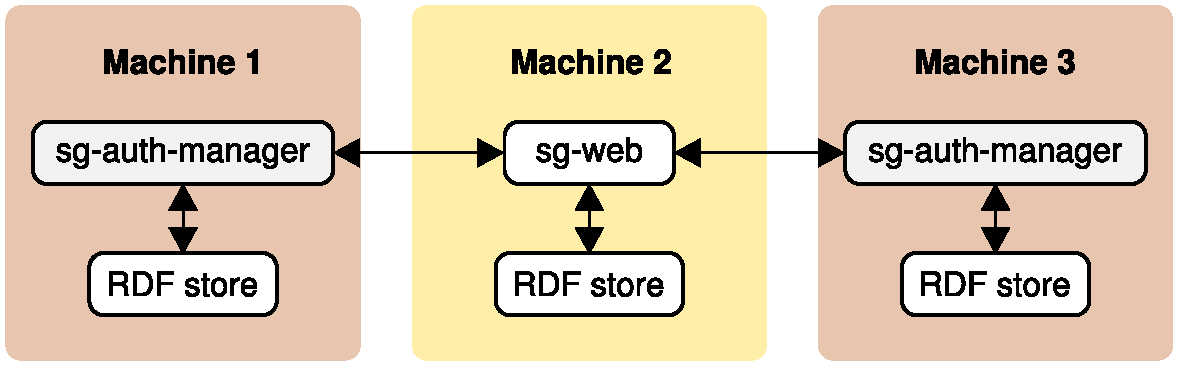
\includegraphics[width=0.8\textwidth]{figures/sg-auth-manager-scaleout.pdf}
    \end{center}
    \caption{\textit{Illustrating a three-node setup.}}
    \label{fig:sg-auth-manager}
  \end{figure}

  %At least one instance of \program{sg-web} must run, so that the
  %\program{sg-auth-manager} can verify the validity of a request that was sent
  %to it.

  The \program{sg-auth-manager} program verifies the validity of the user's session
  token with the \program{sg-web} instance before acting as a proxy to the managed
  RDF store.

\subsection{Importing data into secondary stores}

  RDF importing is handled by an API call to the instance managed by
  \program{sg-auth-manager}.

  When \program{sg-web} receives a request to import data into an
  \program{sg-auth-manager}-managed RDF store, it passes the data directly
  to the \program{sg-auth-manager}, which in turn handles the importing of data
  into that store.

\subsection{How \program{sg-web} handles downtime of a \program{sg-auth-manager}}

  The \program{sg-auth-manager} registers itself with the pre-configured
  \program{sg-web} instance upon start.  In turn, the \program{sg-web} instance
  polls the availability of the \program{sg-auth-manager} instance every 10
  seconds.  When the \program{sg-auth-manager} instance is unavailable for 30
  consecutive seconds, \program{sg-web} removes the connection, and the
  \program{sg-auth-manager} instance must re-register itself.

\subsection{Federated querying of protected endpoints}

  The \t{sg-auth-manager} provides a mechanism to execute federated queries
  using protected endpoints by allowing the session token (see section
  \ref{sec:tokens}) as part of the URI in the \t{SERVICE} specification.

\pagebreak{}
\section{Using the web interface}
\label{sec:using-web-interface}

  Once the web interface is up and running, a logged-in user will land
  on the \i{Dashboard}.

  \begin{figure}[H]
    \begin{center}
      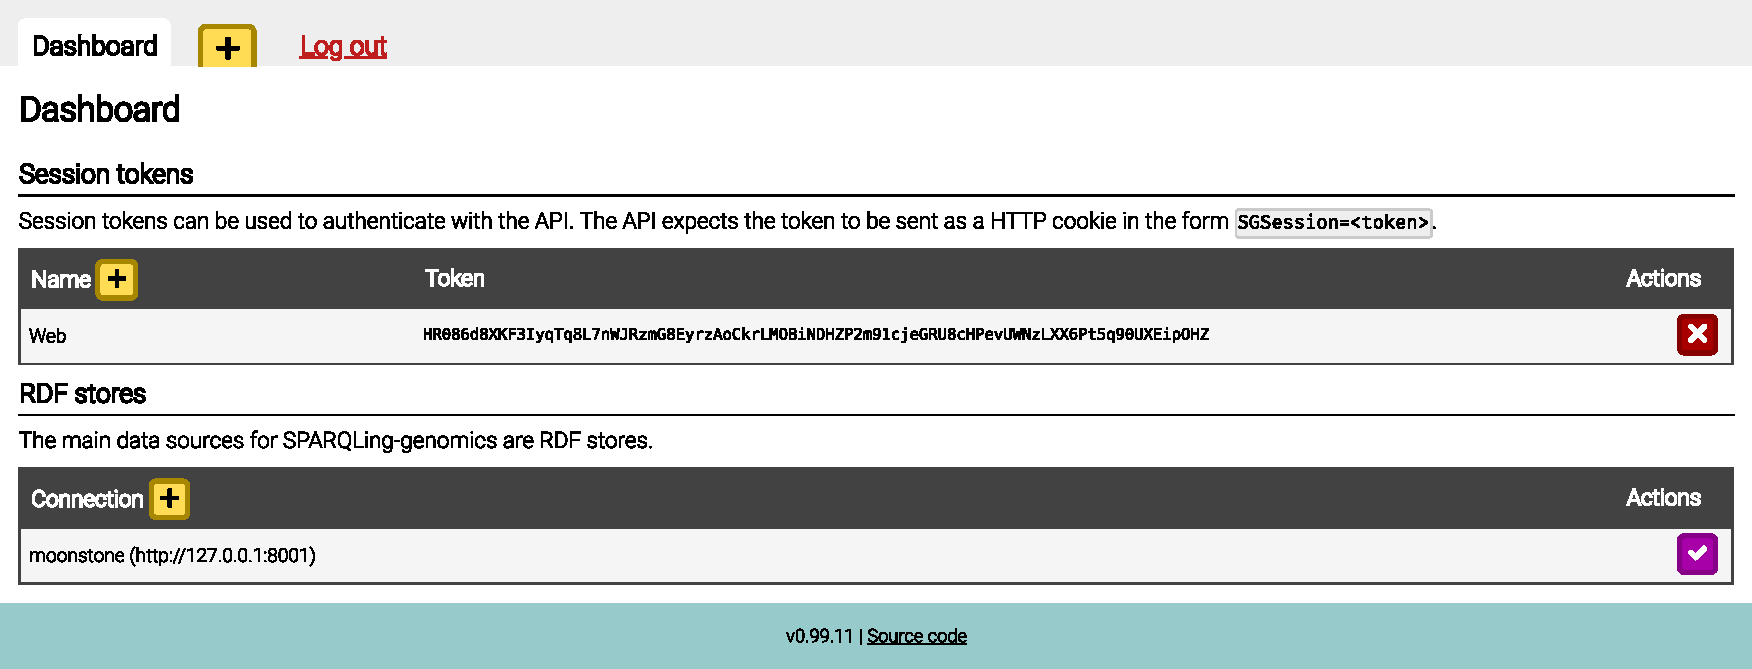
\includegraphics[width=1.0\textwidth]{figures/sg-web-dashboard.pdf}
    \end{center}
    \caption{On the \i{Dashboard}, tokens and connections can be
      configured.}
    \label{fig:web-dashboard}
  \end{figure}

  The dashboard provides access to two resources: \i{session tokens}
  and \i{RDF stores}.  Session tokens will be discussed in section
  \refer{sec:tokens}.  This leaves us with \i{RDF stores} for now.

\subsection{Configuring connections}
\label{sec:configure-connections}

  The web interface supports two types of connections; \i{user-specific
    connections} and \i{system-wide connections}.  Users can add the
  former using the \t{+} button.  Such a connection will only be visible
  to the user who added it.  On the contrary, \i{system-wide connections}
  are visible to all users.

  System-wide connections are therefore not configured by a user, but by a
  program called \program{sg-auth-manager}.  This program works as a middle-man
  between a private RDF store, and a running instance of \program{sg-web}.  It
  uses the user management from \program{sg-web} described in section
  \refer{sec:authentication} to allow users to access graphs assigned to one
  of their projects.

  An instance of \program{sg-auth-manager} registers itself with
  \program{sg-web} as a system-wide connection: making itself available to
  all users of the \program{sg-web} instance.

\subsection{Projects}
\label{sec:web-projects}

  The main way to access the knowledge graph, and to collaborate with other
  users is through a \i{project}.  Projects combine \i{users},
  \i{access to data} and \i{queries}.  The structure of a project
  attempts to capture general phases of analyzing data: \i{collect}
  $\rightarrow$ \i{structure} $\rightarrow$ \i{query} $\rightarrow$
  \i{report} $\rightarrow$ \i{automate}.

  \begin{figure}[H]
    \begin{center}
      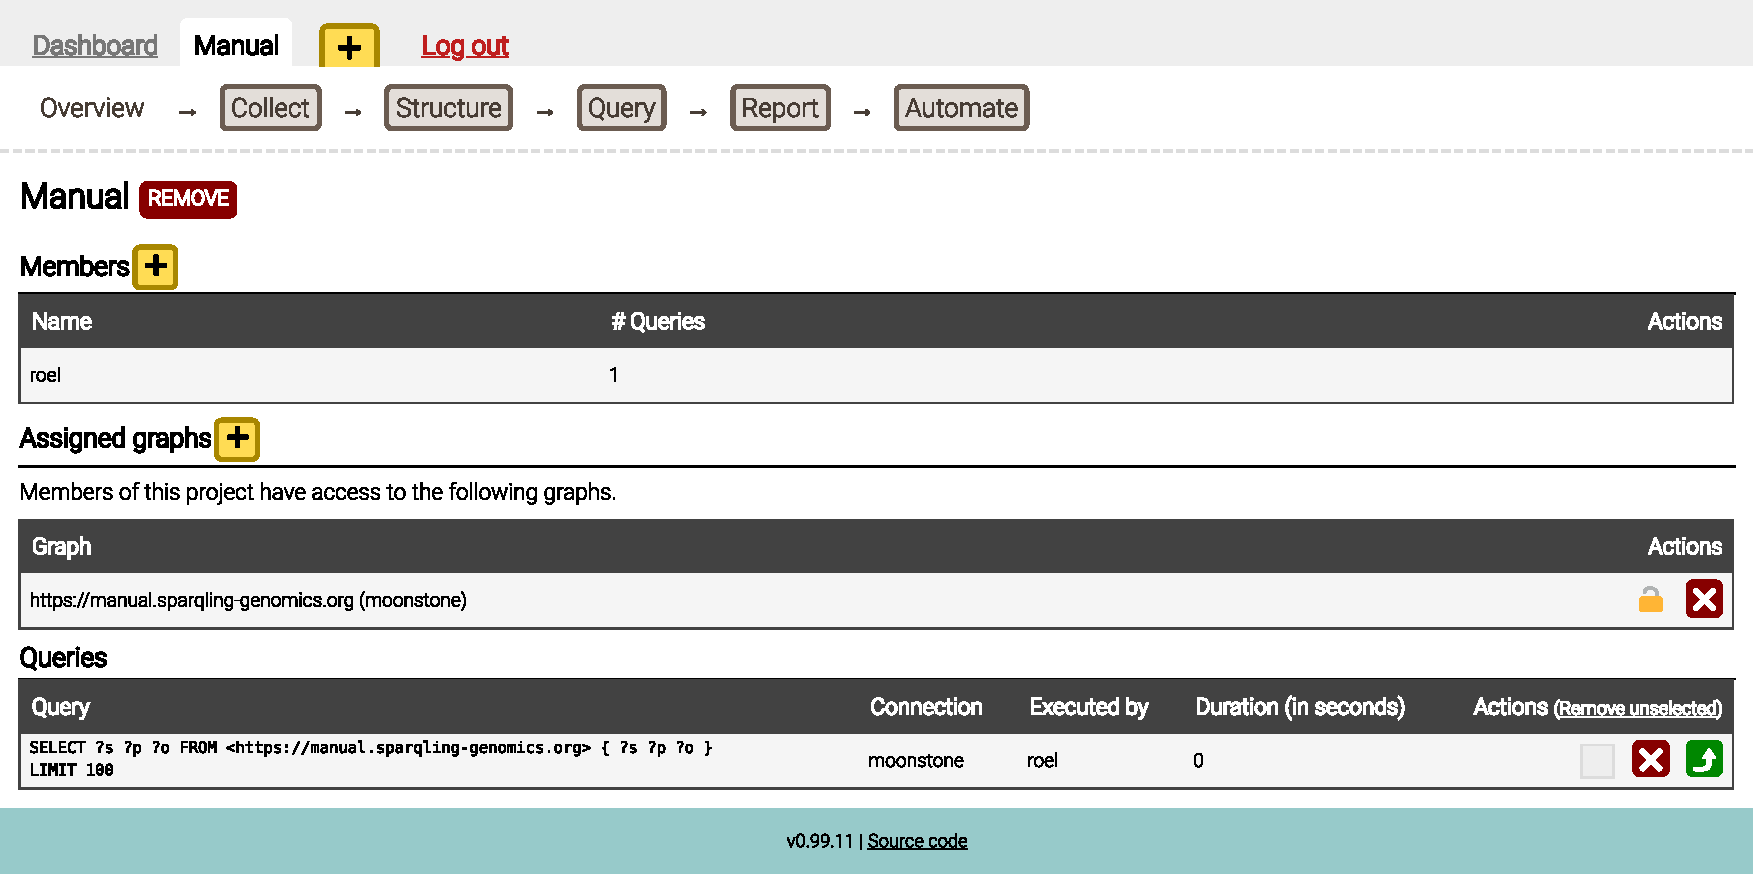
\includegraphics[width=1.0\textwidth]{figures/sg-web-project-details.pdf}
    \end{center}
    \caption{The project overview page.}
    \label{fig:web-project-overview}
  \end{figure}

\subsubsection{Collecting data}

  Before data can be analyzed, it must be collected and stored.  Graphs are
  the primary place to store data.  Graphs are identified by a uniform resource
  identifier (URI).  So before data can be imported, a project must assign a
  graph.

  After assigning a graph to the project on the \i{Overview} page, the
  command to load a file can be generated in three steps.

  \begin{figure}[H]
    \begin{center}
      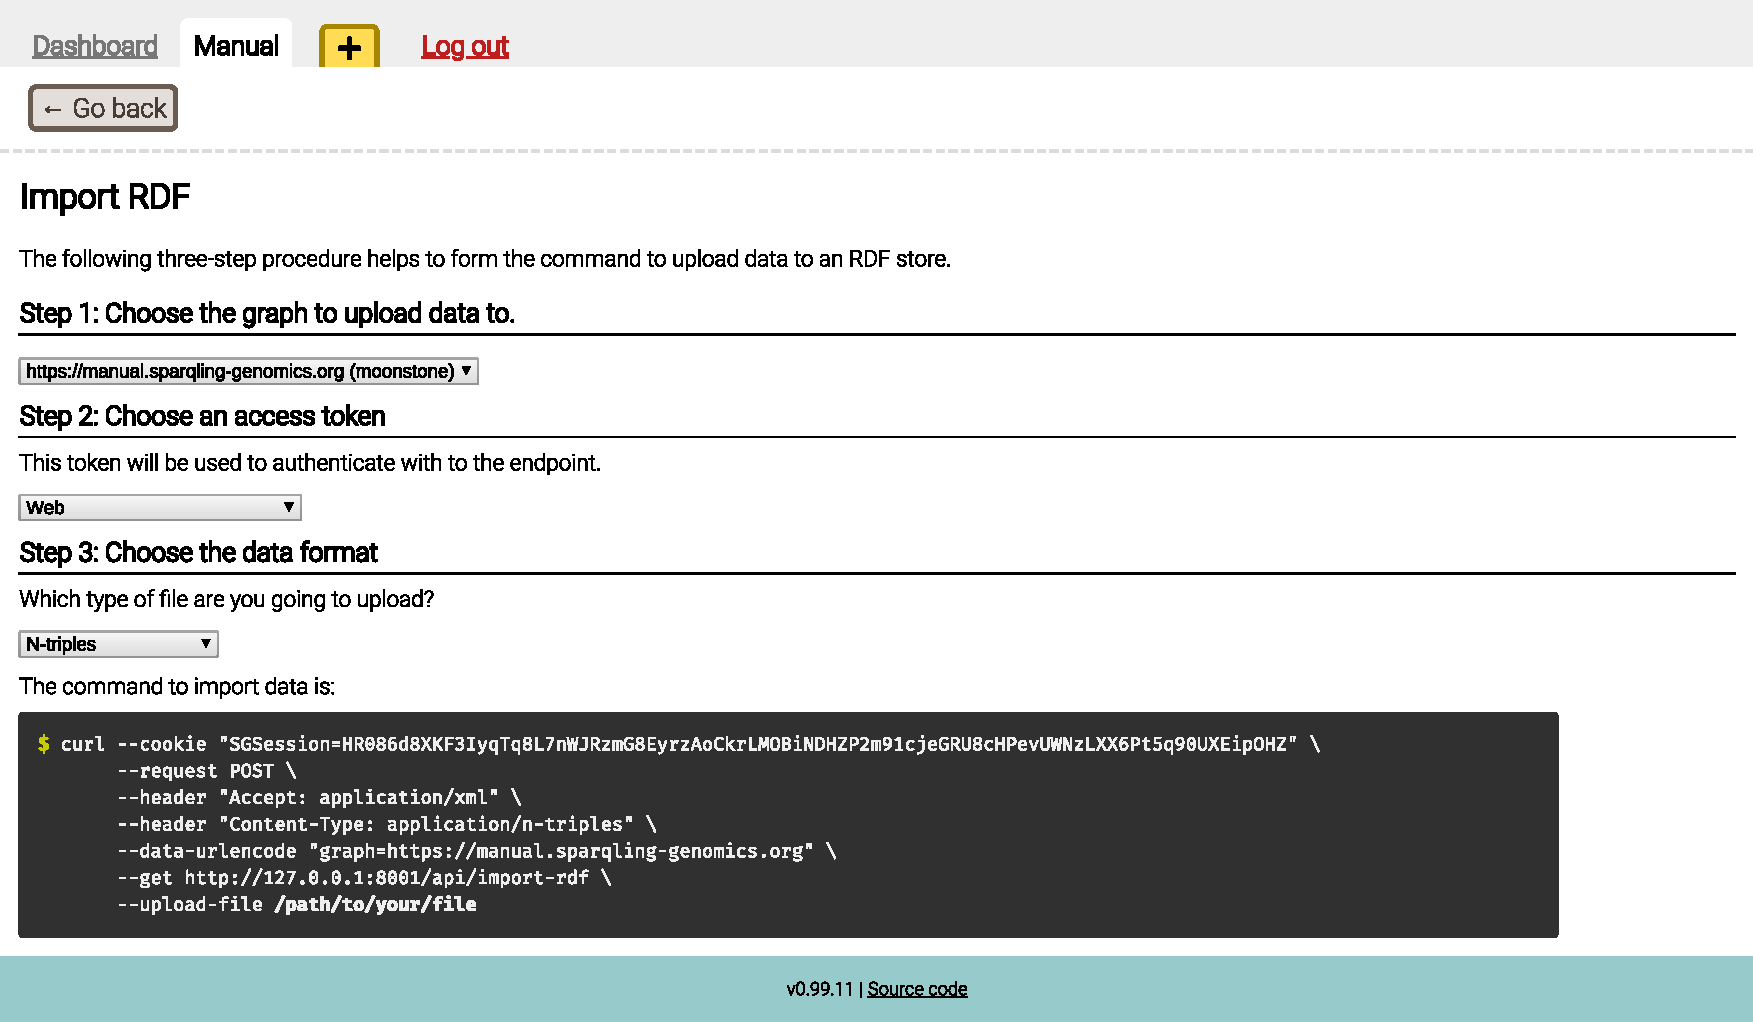
\includegraphics[width=1.0\textwidth]{figures/sg-web-import-rdf.pdf}
    \end{center}
    \caption{Importing RDF in three steps}
    \label{fig:web-import-rdf}
  \end{figure}

\subsection{Executing queries}

  After configuring at least one endpoint, it can be chosen on the \i{query}
  page to execute a query against it.

  \begin{figure}[H]
    \begin{center}
      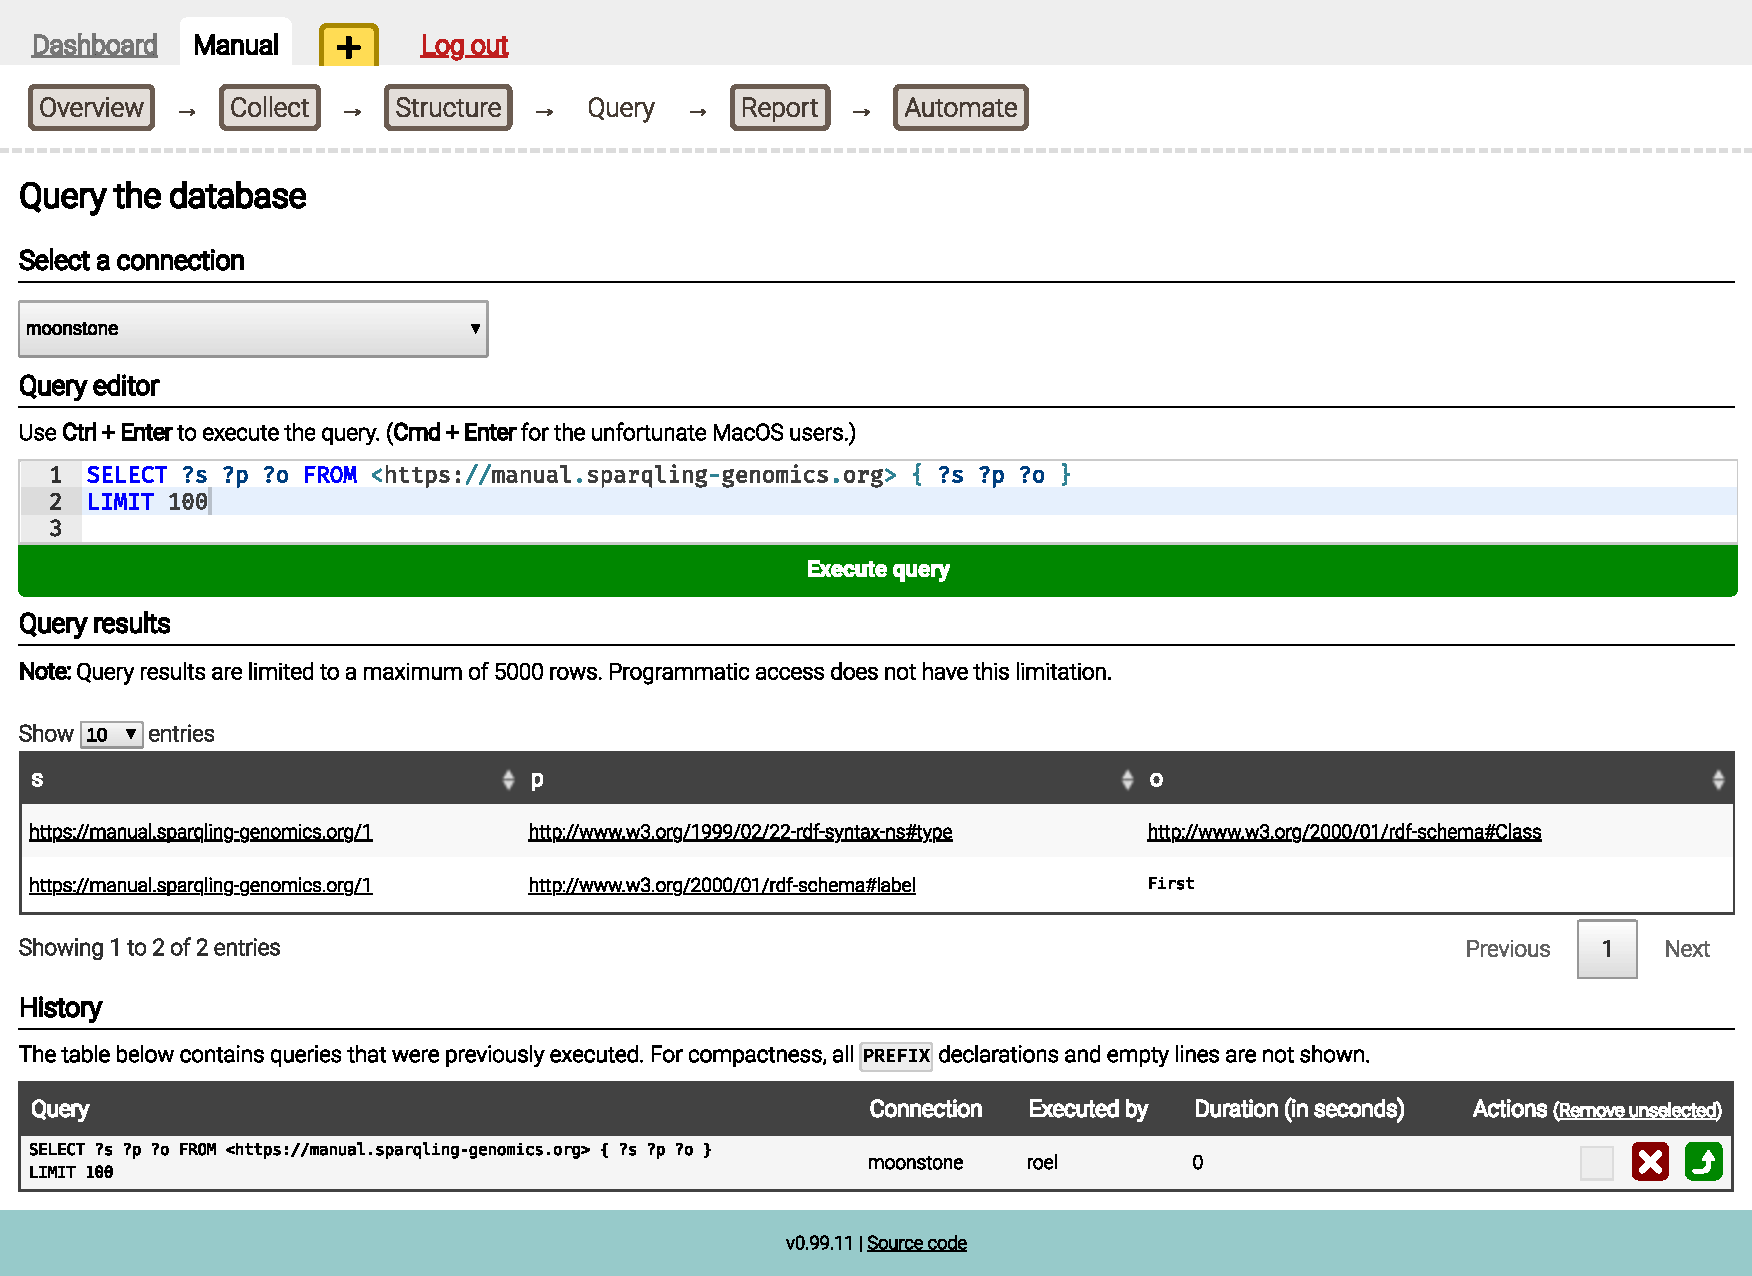
\includegraphics[width=1.0\textwidth]{figures/sg-web-query.pdf}
    \end{center}
    \caption{The \i{query} page enables users to execute a query against a
      SPARQL endpoint.  The connections configured at the \i{connections} page
      can be chosen from the drop-down menu.}
    \label{fig:web-query}
  \end{figure}

\subsection{Query history}
\label{sec:query-history}

  When prototyping SPARQL queries, better known as ``SPARQLing around'', it's
  good to know that all queries that yielded a result are stored in the
  \i{query history}.  The history is shown on the \i{query} page below the
  query editor.  Each \i{project} has its own query history.

\subsection{Explore graphs with the Exploratory}

  Another utility aimed at SPARQLing around faster is the \i{exploratory}.

  \begin{figure}[H]
    \begin{center}
      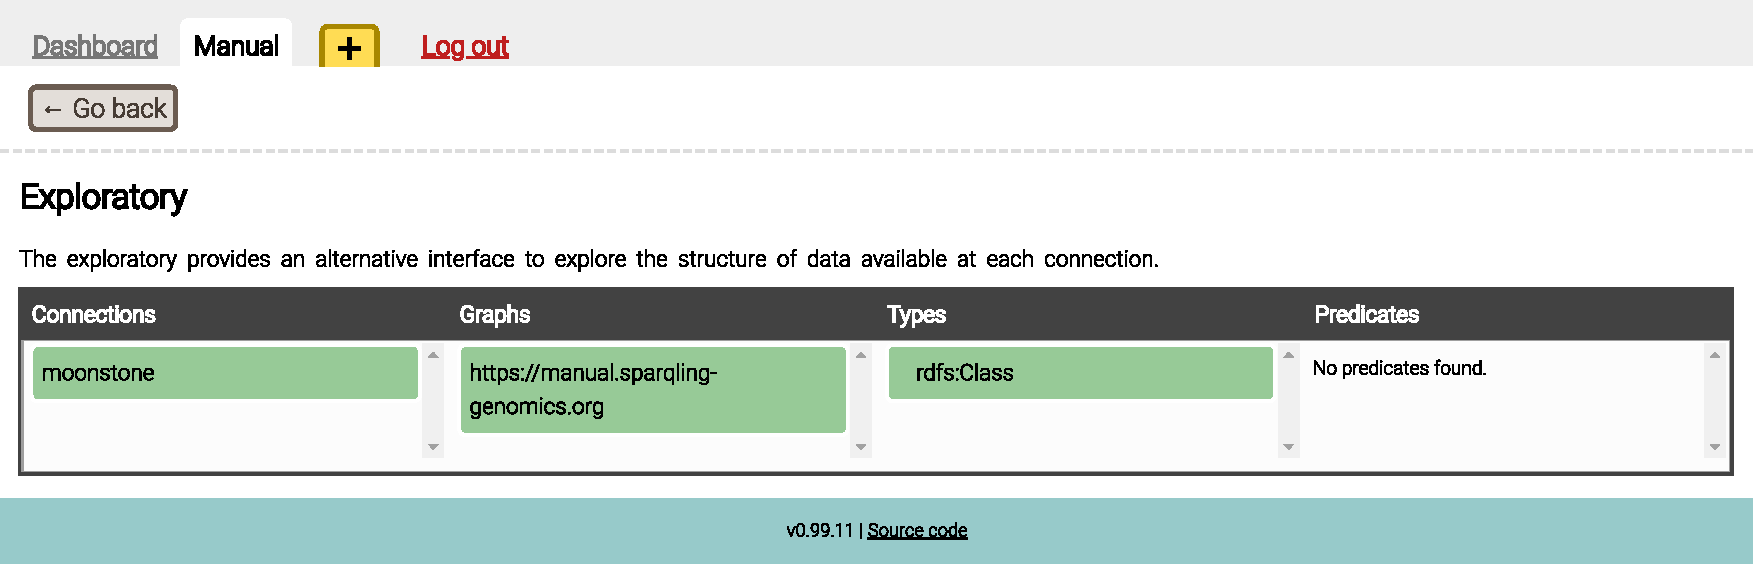
\includegraphics[width=1.0\textwidth]{figures/sg-web-exploratory.pdf}
    \end{center}
    \caption{The \i{exploratory} page enables users to learn about the
      structure of the triplets in a graph.}
    \label{fig:web-exploratory}
  \end{figure}

  The exploratory uses a common pattern in RDF to help writing queries.  Its
  interface provides a four-step selection process to find \i{predicates}
  associated with an \t{rdf:type}.  The programs described in chapter
  \refer{chap:command-line} automatically add the \t{rdf:type} annotations.

\subsection{Connections and graphs}

  The first step in finding predicates involves choosing a connection
  (see section \refer{sec:configure-connections}).  The second step involves
  choosing a graph.  If the connection does not support the use of graphs,
  the journey ends here.

\subsection{Types}

  The third step looks for triplets that match the pattern \i{subject}
  $\rightarrow$ \t{rdf:type} $\rightarrow$ \i{type}.  All matches for
  \i{type} are displayed.  For data imported with \t{vcf2rdf} (see
  section \refer{sec:vcf2rdf}), this will display (among other types) the
  \t{VariantCall} type.

\subsection{Predicates}

  Staying with the \t{VariantCall} example;  All data properties extracted
  from a VCF file can be found under this type.  A predicate displayed in this
  column occurs in \i{at least} one triplet.  It not necessarily occurs in
  \i{every} triplet.  Especially when using \t{INFO} and \t{FORMAT}
  fields in a VCF file, we recommend using them in a query inside an
  \t{OPTIONAL} clause.

\pagebreak{}
\section{Programming interface}
\label{sec:web-api}

  Other than a user interface, the web interface provides a programming interface
  using the HyperText Transport Protocol (HTTP).  The interface supports XML,
  JSON, and S-expressions.  Table \ref{table:api-return-formats} summarizes the
  supported formats.

  \hypersetup{urlcolor=black}
  \begin{table}[H]
    \begin{tabularx}{\textwidth}{l!{\VRule[-1pt]}X}
      \headrow
      \b{Content-Type} & \b{Example response}\\
      \evenrow
      \t{application/json}
      & \t{[\{ "message": "This is a JSON response." \}]}\\
      \oddrow
      \t{application/xml}
      & \t{<message>This is a XML response.</message>}\\
      \evenrow
      \t{application/s-expression}
      & \t{(message . "This is a S-expression response.")}\\
    \end{tabularx}
    \caption{\small Implemented content types for the API.  The
      \t{Content-Type} can be used in the \t{Accept} HTTP header.}
    \label{table:api-return-formats}
  \end{table}
  \hypersetup{urlcolor=LinkGray}

\subsection{Formatting \t{POST} requests}

  The \t{Accept} parameter influences the response format of the API,
  and the \t{Content-Type} parameter can be used to indicate the format
  of the request.

  In addition to the documented \t{Content-Type} values, the type
  \t{application/x-www-form-urlencoded} is also allowed, which expects
  the following format:
\begin{siderules}
\begin{verbatim}
parameter1=value1&parameter2=value2&...
\end{verbatim}
\end{siderules}

  The \t{Content-Type} header line does not have to be equal to the
  \t{Accept} header line, so for example, parameters can be sent in
  XML and the response can be formatted in JSON or the other way around.

\subsection{Conventions when using XML}

\begin{sloppypar}
  When using XML, there are a few conventions to follow.  To communicate a list
  or array of records, the API relies on using pre-defined elements. The API
  expects parameters to be wrapped in \t{<parameters>...</parameters>}
  elements.  So, to log in using an XML request, the following message will be
  accepted:
\end{sloppypar}

\begin{siderules}
\begin{verbatim}
POST /api/login HTTP/1.1
Host: ...
Content-Type: application/xml
Content-Length: 80
Connection: close

<parameters>
  <username>...</username>
  <password>...</password>
</parameters>
\end{verbatim}
\end{siderules}

  Subsequently, when \t{Accept}ing XML the results are wrapped in
  \t{<results>...</results>}, and data structures built from multiple
  key-value pairs are wrapped in \t{<result>...<result>}.  The
  following example illustrates receiving a project record:

\begin{siderules}
\begin{verbatim}
GET /api/projects HTTP/1.1
Host: ...
Accept: application/xml
Cookie: ...
Connection: close

<results>
  <result>
    <projectId>http://sparqling-genomics.org/0.99.10/Project/...</projectId>
    <creator>http://sparqling-genomics.org/0.99.10/Agent/...</creator>
    ...
  </result>
</results>
\end{verbatim}
\end{siderules}

\b{Note}: The actual response strips the whitespace.  It was added to
this example for improved readability.

\subsection{Authenticating API requests with \t{/api/login}}
\label{sec:api-login}

  Before being able to interact with the API, a session token must be obtained.
  This can be done by sending a \t{POST}-request to \t{/api/login},
  with the following parameters:

  \hypersetup{urlcolor=black}
  \begin{table}[H]
    \begin{tabularx}{\textwidth}{l!{\VRule[-1pt]}X!{\VRule[-1pt]}X}
      \headrow
      \b{Parameter} & \b{Example} & \b{Required?}\\
      \evenrow
      \t{username}  & \t{jdoe}    & Yes\\
      \oddrow
      \t{password}  & \t{secret}  & Yes\\
    \end{tabularx}
  \end{table}
  \hypersetup{urlcolor=LinkGray}

  The following cURL command would log the user \t{jdoe} in:

\begin{siderules}
\begin{verbatim}
curl --cookie-jar - http://localhost/api/login \
     --data "username=jdoe&password=secret"
\end{verbatim}
\end{siderules}

  The response contains a cookie with the session token.  Use this cookie in
  subsequent requests.  When authentication fails, the service will respond
  with HTTP status-code \t{401}.

\subsection{Token-based authentication}
\label{sec:tokens}

  When automating data importing and running queries there comes the point
  at which you have a choice: Do I put in my login credentials in a script,
  a separate file, or anywhere else on the filesystem?  This bad security
  practice can be overcome by using \i{tokens}.

  A token is a randomly generated string that can be used to authenticate
  with, instead of your username and password.  Tokens are easy to create,
  and more importantly, easy to revoke.

  Generating a token can be done on the \i{Dashboard}, or using the API call
  \t{/api/new-session-token}.  Removing a token can be done on the
  \i{Dashboard}, or using the API call \t{/api/delete-token}.

  After generating a token, it can be used as a cookie in API calls.  The name
  of the cookie is always \t{SGSession}, regardless of the name of the
  token.

\subsection{Managing connections}

  The API can be used to store connections and refer to them by name.  The
  remainder of this section describes the API calls related to connections.

\subsubsection{Retrieve connections with \t{/api/connections}}

  With a call to \t{/api/connections}, the pre-configured connections
  can be viewed.  This resource expects a \t{GET} request and needs no
  parameters.  It returns all connection records associated with the currently
  logged-in user.

  The following cURL command would retrieve all connection records in JSON
  format:

\begin{siderules}
\begin{verbatim}
curl http://localhost/api/connections \
     --cookie "$COOKIE"               \
     -H "Accept: application/json"
\end{verbatim}
\end{siderules}

\subsubsection{Create a new connection with \t{/api/add-connection}}
\label{sec:api-create-connection}

  A call to \t{/api/add-connection} will create a new connection.
  The table below summarizes the parameters that can be used in this call.

  \hypersetup{urlcolor=black}
  \begin{table}[H]
    \begin{tabularx}{\textwidth}{l!{\VRule[-1pt]}X!{\VRule[-1pt]}X}
      \headrow
      \b{Parameter} & \b{Example}            & \b{Required?}\\
      \evenrow
      \t{name}      & \t{Example}            & Yes\\
      \oddrow
      \t{uri}       & \t{http://my/endpoint} & Yes\\
      \evenrow
      \t{username}  & \t{jdoe}               & No\\
      \oddrow
      \t{password}  & \t{secret}             & No\\
      \evenrow
      \t{backend}   & \t{4store}             & No\\
    \end{tabularx}
  \end{table}
  \hypersetup{urlcolor=LinkGray}

  The following cURL command would create a connection, using JSON as
  the format to express the parameters:

\begin{siderules}
\begin{verbatim}
curl http://localhost/api/add-connection          \
     --cookie "$COOKIE"                           \
     -H "Accept: application/xml"                 \
     -H "Content-Type: application/json"          \
     --data '{ "name":     "Example",             \
                "uri":      "http://my/endpoint", \
                "username": "jdoe",               \
                "password": "secret",             \
                "backend":  "4store" }'
\end{verbatim}
\end{siderules}

\subsubsection{Remove a connection with \t{/api/remove-connection}}

  A call to \t{/api/remove-connection} will remove an existing
  connection.  The table below summarizes the parameters that can be
  used in this call.

  \hypersetup{urlcolor=black}
  \begin{table}[H]
    \begin{tabularx}{\textwidth}{l!{\VRule[-1pt]}X!{\VRule[-1pt]}X}
      \headrow
      \b{Parameter} & \b{Example} & \b{Required?}\\
      \evenrow
      \t{name}      & \t{Example} & Yes\\
    \end{tabularx}
  \end{table}
  \hypersetup{urlcolor=LinkGray}

  The following cURL command would remove the connection that was created in
  section \refer{sec:api-create-connection}:

\begin{siderules}
\begin{verbatim}
curl http://localhost/api/remove-connection       \
     --cookie "$COOKIE"                           \
     -H "Accept: application/xml"                 \
     --data "name=Example"
\end{verbatim}
\end{siderules}

\subsection{Managing projects}

  The API has various resources to manage projects, as described in
  section \refer{sec:web-projects}.

\subsubsection{Retrieve a list of projects with \t{/api/projects}}

  Retrieving a list of projects can be done by sending a \t{GET} request
  to \t{/api/projects}.

  The following cURL command would retrieve a list of projects:

\begin{siderules}
\begin{verbatim}
curl http://localhost/api/projects      \
     --cookie "$COOKIE"                 \
     -H "Accept: application/xml"
\end{verbatim}
\end{siderules}

\subsubsection{Create a new project with \t{/api/add-project}}
\label{sec:api-add-project}

  To create a new project, send a \t{POST} request to
  \t{/api/add-project}.  The table below summarizes the parameters
  that can be used with this call.

  \hypersetup{urlcolor=black}
  \begin{table}[H]
    \begin{tabularx}{\textwidth}{l!{\VRule[-1pt]}X!{\VRule[-1pt]}X}
      \headrow
      \b{Parameter} & \b{Example}         & \b{Required?}\\
      \evenrow
      \t{name}      & \t{Example project} & Yes\\
    \end{tabularx}
  \end{table}
  \hypersetup{urlcolor=LinkGray}

  The following cURL command would add a project:

\begin{siderules}
\begin{verbatim}
curl http://localhost/api/add-project      \
     --cookie "$COOKIE"                    \
     -H "Accept: application/xml"          \
     --data "name=Example project"
\end{verbatim}
\end{siderules}

\subsubsection{Remove a project with \t{/api/remove-project}}

  To remove a project, send a \t{POST} request to
  \t{/api/remove-project}.  The table below summarizes the parameters
  that can be used with this call.

  \hypersetup{urlcolor=black}
  \begin{table}[H]
    \begin{tabularx}{\textwidth}{l!{\VRule[-1pt]}l!{\VRule[-1pt]}X}
      \headrow
      \b{Parameter}   & \b{Example} & \b{Required?}\\
      \evenrow
      \t{project-uri}
      & \t{http://sparqling-genomics.org/Project/640c0...5a6d2} & Yes\\
    \end{tabularx}
  \end{table}
  \hypersetup{urlcolor=LinkGray}

  Alternatively, instead of the full URI, the project's hash can be used.
  In that case, the parameters are:

  \hypersetup{urlcolor=black}
  \begin{table}[H]
    \begin{tabularx}{\textwidth}{l!{\VRule[-1pt]}l!{\VRule[-1pt]}X}
      \headrow
      \b{Parameter}    & \b{Example}       & \b{Required?}\\
      \evenrow
      \t{project-hash} & \t{640c0...5a6d2} & Yes\\
    \end{tabularx}
  \end{table}
  \hypersetup{urlcolor=LinkGray}

  The following cURL command would remove the project created in
  \refer{sec:api-add-project}:

\begin{siderules}
\begin{verbatim}
curl http://localhost/api/remove-project      \
     --cookie "$COOKIE"                       \
     -H "Accept: application/xml"             \
     --data "project-uri=http://sparqling-genomics.org/Project/640c0...5a6d2"
\end{verbatim}
\end{siderules}

\subsubsection{Assign a graph to a project \t{/api/assign-graph}}

  Assigning a graph to a project can be done by sending a \t{POST} request
  to \t{/api/assign-graph}.  The required parameters are:

  \begin{itemize}
    \item{\t{project-uri}: This can be obtained from a call to
      \t{/api/projects}.}
    \item{\t{connection}: The name of a connection obtained from
      a call to \t{/api/connections}.}
    \item{\t{graph-uri}: The graph URI to assign.}
  \end{itemize}

  The following example based on cURL shows how to perform the request:
\begin{siderules}
\begin{verbatim}
curl -X POST                                               \
     -H "Accept: application/json"                         \
     -H "Content-Type: application/json"                   \
     --cookie "SGSession=..."                              \
     --data '{ "project-uri": "http://the-project-uri",    \
               "connection": "wikidata",                   \
               "graph-uri": "http://the-new-graph-name" }' \
     http://localhost/api/assign-graph
\end{verbatim}
\end{siderules}

\subsubsection{Unassign a graph from a project with \t{/api/unassign-graph}}

  Like assigning a graph to a project, it can be unassigned as well using
  \t{/api/unassign-graph} using the same parameters as
  \t{/api/assign-graph}.

  The following example based on cURL shows how to perform the request:
\begin{siderules}
\begin{verbatim}
curl -X POST                                               \
     -H "Accept: application/json"                         \
     -H "Content-Type: application/json"                   \
     --cookie "SGSession=..."                              \
     --data '{ "project-uri": "http://the-project-uri",    \
               "graph-uri": "http://the-new-graph-name" }' \
     http://localhost/api/unassign-graph
\end{verbatim}
\end{siderules}

\pagebreak{}
\subsection{Running and viewing queries}

\subsubsection{Retrieve previously run queries with \t{/api/queries}}

  When running queries through SPARQLing-genomics's interface, each succesful
  query is stored in a ``query history''.  This query history can be retrieved
  using a call to \t{/api/queries}.  This resource expects a \t{GET}
  request.

  The following cURL command would retrieve the entire query history, formatted
  as XML:

\begin{siderules}
\begin{verbatim}
curl http://localhost/api/queries \
     --cookie "$COOKIE"           \
     -H "Accept: application/xml"
\end{verbatim}
\end{siderules}

\subsubsection{Toggle query marks}

\begin{sloppypar}
  Previously executed queries can be marked as \i{important}, which means
  they will survive a call to \t{/api/queries-remove-unmarked}.
\end{sloppypar}

  The following example based on cURL shows how to mark a query as
  \i{important}:
\begin{siderules}
\begin{verbatim}
curl -X POST                                               \
     -H "Accept: application/json"                         \
     -H "Content-Type: application/json"                   \
     --cookie "SGSession=..."                              \
     --data '{ "query-id": "...", "state": true }'
     http://localhost/api/query-mark
\end{verbatim}
\end{siderules}

\subsubsection{Remove unmarked queries}

  Removing unmarked queries for a project can be done by sending a
  \t{POST} request to \t{/api/queries-remove-unmarked}.
  The required parameters are:

  \begin{itemize}
    \item{\t{project-uri}: This can be obtained from a call to
      \t{/api/projects}.}
  \end{itemize}

  The following example based on cURL shows how to perform the request:
\begin{siderules}
\begin{verbatim}
curl -X POST                                               \
     -H "Accept: application/json"                         \
     -H "Content-Type: application/json"                   \
     --cookie "SGSession=..."                              \
     --data '{ "project-uri": "http://the-project-uri" }'
     http://localhost/api/queries-remove-unmarked
\end{verbatim}
\end{siderules}

\pagebreak{}
\section{Forms}
\label{sec:forms}

  The \program{sg-web} program can be extended to provide a web form interface.
  Creating a web form that leverages SPARQLing-genomics involves creating a
  Scheme module that implements three procedures:
  \begin{itemize}
  \item \t{page}: This procedure should return an SXML tree that represents
    the HTML to display the form.
  \item \t{submit}: This function implements the action to take when a user
    submits the form.
  \item \t{api}: This optional function can be used to build autocompletion,
    or other pre-submit interaction between the form and SPARQLing-genomics.
  \end{itemize}

\subsection{Example of a form module}

  Creating a Scheme module to render a form to users comprises of four
  parts.  In the remainder of this section we will address each part.

\subsubsection{The Scheme module}

  The first part involves defining a Scheme modules with three procedures.
  Because \program{sg-web} is written in GNU Guile \citep{guile},
  we use \t{define-module} to define the module for the form.

\begin{siderules}
\begin{verbatim}
(define-module (www forms example)
  #:use-module (www pages) ; Provides the ‘page-empty-template’ procedure.
  #:use-module (www util)  ; Provides the ‘string-is-longer-than’ procedure.
  #:export (page submit api))
\end{verbatim}
\end{siderules}

  Because the name of the module is \t{(www forms example)}, the location
  where \program{sg-web} searches for your module is `\t{www/forms/example.scm}'
  relative to a path on \t{GUILE\_LOAD\_PATH}.  The ``\t{www form}'' module
  prefix is hard-coded by \program{sg-web}, while \t{example} can be chosen by
  us.

  There are three symbols we export from our module: \t{page}, \t{submit}, and
  \t{api}.  The \program{sg-web} expects these exact symbol names to be
  exported.

\subsubsection{Implementing the \t{page} procedure}

  The second part involves implementing the \t{page} procedure. The \t{page}
  procedure takes the request path as argument (ignoring optional arguments),
  returning an SXML tree.  The request path can be used to tell where to
  submit the form to.

\begin{siderules}
\begin{verbatim}
(define* (page request-path #:optional (error-message #f))
  (page-empty-template "Example" request-path
   `((h2 "Example form")
     ,(if error-message
         `(div (@ (class "form-error-message")) ,error-message)
         '())

     (form (@ (method "POST")
              (action ,request-path))
       (h3 "Name")
       (input (@ (type  "text")
                 (id    "name")
                 (name  "name")))
       (input (@ (type  "submit")
                 (class "form-submit-button")
                 (value "Submit form")))))))
\end{verbatim}
\end{siderules}

  The \t{(www pages)} module provides a template that includes the familiar
  theme of the \program{sg-web} pages.  Our SXML tree will render to the
  following HTML:

\begin{siderules}
\begin{verbatim}
<h2>Example form</h2>
<form method="POST" action="/forms/example">
  <h3>Name</h3>
  <input type="text" id="name" name="name" />
  <input type="submit" class="form-submit-button" value="Submit form" />
</form>
\end{verbatim}
\end{siderules}

  Note that this HTML snippet is wrapped inside the template constructed by
  \t{page-empty-template}, so when viewing the form in a web browser, we
  will see something similar to figure \ref{fig:web-form-example}.

  \begin{figure}[H]
    \begin{center}
      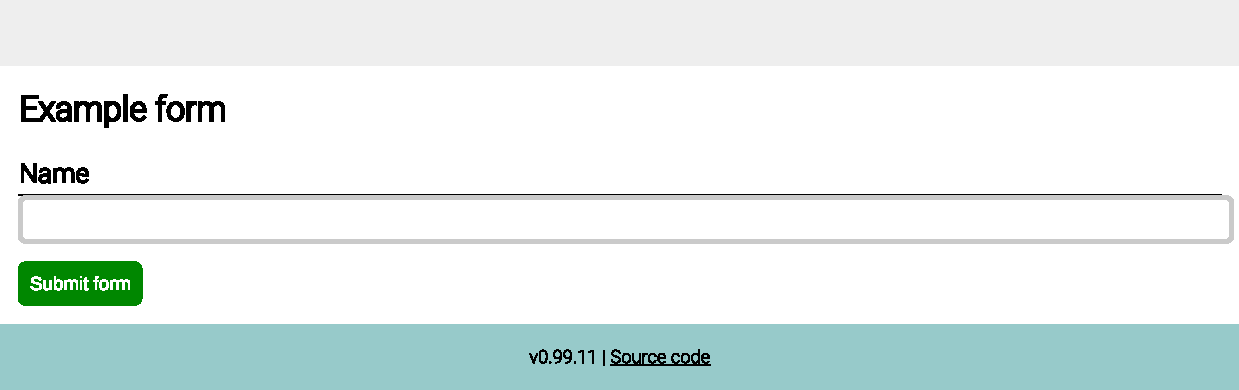
\includegraphics[width=1.0\textwidth]{figures/sg-web-form-example.pdf}
    \end{center}
    \caption{The rendering of the \t{page} function of our example form.}
    \label{fig:web-form-example}
  \end{figure}

\subsubsection{Implementing the \t{submit} procedure}

  Our next step is to catch a form submission, which is the purpose of the
  \t{submit} procedure.  This procedure is expected to take two arguments,
  and return an SXML tree.

\begin{siderules}
\begin{verbatim}
(define (submit request-path data)
  (let* ((name (assoc-ref data 'name))
         (state (cond
                 [(or (not name)
                      (not (string-is-longer-than name 0)))
                  '(#f "Missing name.")]
                 [(string-is-longer-than name 64)
                  '(#f "Name may not be longer than 64 characters.")]
                 [else
                  '(#t)])))
    (if (car state)
        (page-empty-template "Thank you" request-path
         `((h2 "Thank you, " ,name "!")))
        (page request-path (cadr state)))))
\end{verbatim}
\end{siderules}

  After submitting the form, it may render in the web browser as displayed
  in figure \ref{fig:web-form-submit}.

  \begin{figure}[H]
    \begin{center}
      
\includegraphics[width=1.0\textwidth]{figures/sg-web-form-example-submit.pdf}
    \end{center}
    \caption{The rendering of the \t{submit} function of our example form.}
    \label{fig:web-form-submit}
  \end{figure}


\subsubsection{Implementing the \t{api} procedure}

  The final part involves implementing the optional \t{api} procedure
  takes six arguments:
  \begin{itemize}
  \item \t{request-path}:   The relative path of the form;
  \item \t{input-port}:     The port to read data from;
  \item \t{output-port}:    The port to write data to;
  \item \t{accept-type}:    The value of the requests's \t{Accept} header;
  \item \t{content-type}:   The value of the requests's \t{Content-Type} header;
  \item \t{content-length}: The number of bytes that can be read from
    \t{input-port}.
  \end{itemize}

  This procedure is primarily designed to provide autocompletion options
  for form fields.

\begin{siderules}
\begin{verbatim}
(define (api request-path input-port output-port
             accept-type content-type content-length)
  ...)
\end{verbatim}
\end{siderules}


\ifdefined\HCode
\begin{html}
</div></div><div class="chapter"><div class="chapwrap">
\end{html}
\fi

\chapter{Information retrieval with SPARQL}
\label{chap:information-retrieval}

  In section \refer{sec:vcf2rdf} we discussed how to extract triples from
  common data formats.  In section \refer{sec:curl} we discussed how we
  could insert those triples into a SPARQL endpoint.

  In this section, we will start exploring the inserted data by using a
  query language called \i{SPARQL}.  Understanding SPARQL will be crucial
  for the integration in our own programs or scripts --- something we will
  discuss in chapter \refer{chap:programming}.

  The queries in the remainder of this chapter can be readily copy/pasted into
  the query editor of the web interface (see chapter
  \refer{chap:web-interface}).

\section{Local querying}

  When we request information from a SPARQL endpoint, we are performing a
  \i{local query} because we request data from a single place.  In our case,
  that is most likely to be our own SPARQL endpoint.

  In contrast to \i{local querying}, we can also query multiple SPARQL
  endpoints in one go, to combine the information from multiple locations.
  Combining information from multiple SPARQL endpoints is called \i{federated
    querying}.

  Federated querying is discussed in section \refer{sec:federated-querying}.

\subsection{Listing non-empty graphs}
\label{sec:non-empty-graphs}
  Each SPARQL endpoint can host multiple \i{graphs}.  Each graph can contain
  an independent set of triples.  The following query displays the available
  non-empty graphs in a SPARQL endpoint:

\begin{lstlisting}[language=SPARQL]
SELECT DISTINCT ?graph WHERE { GRAPH ?graph { ?s ?p ?o } }
\end{lstlisting}

Which may yield the following table:

\begin{table}[H]
  \begin{tabularx}{\textwidth}{ L }
    \headrow
    \b{graph}\\
    \evenrow
    \t{http://example}\\
    \oddrow
    \t{http://localuriqaserver/sparql}\\
    \evenrow
    \t{http://www.openlinksw.com/schemas/virtrdf\#}\\
    \oddrow
    \t{http://www.w3.org/2002/07/owl\#}\\
    \evenrow
    \t{http://www.w3.org/ns/ldp\#}\\
  \end{tabularx}
  \caption{\small Results of the query to list non-empty graphs.}
  \label{table:query-output-1}
\end{table}

  The graph names usually look like URLs, like we would encounter them on the
  web.  In fact, not only graph names, but any node that has a symbolic meaning,
  rather than a literal\footnote{Examples of literals are numbers and strings.
    Symbols are nodes that don't have a literal value.} meaning is usually
  written as a URL.  We can go to such a URL with a web browser and might even
  find more information.

\subsection{Querying a specific graph}

  The sooner we can reduce the dataset to query over, the faster the query will
  return with an answer.  One easy way to reduce the size of the dataset is to
  be specific about which graph to query.  This can be achieved using the
  \t{FROM} clause in the query.

\begin{lstlisting}[language=SPARQL]
SELECT ?s ?p ?o
FROM <graph-name>
WHERE { ?s ?p ?o }
\end{lstlisting}

  The \t{graph-name} must be one of the graphs returned by the query from
  section \refer{sec:non-empty-graphs}.

  Without the \t{FROM} clause, the RDF store will search in all graphs.
  We can repeat the \t{FROM} clause to query over multiple graphs in the
  same RDF store.

\begin{lstlisting}[language=SPARQL]
SELECT ?s ?p ?o
FROM <graph-name>
FROM <another-graph-name>
WHERE { ?s ?p ?o }
\end{lstlisting}

  In section \refer{sec:federated-querying} we will look at querying over
  multiple RDF stores.

\subsection{Exploring the structure of knowledge in a graph}


  Inside the \t{WHERE} clause of a SPARQL query we specify a graph
  pattern.  When the information in a graph is structured, there are only few
  predicates in comparison to the number of subjects and the number of objects.

\begin{lstlisting}[language=SPARQL]
SELECT COUNT(DISTINCT ?s) AS ?subjects
       COUNT(DISTINCT ?p) AS ?predicates
       COUNT(DISTINCT ?o) AS ?objects
FROM <http://example>
WHERE { ?s ?p ?o }
\end{lstlisting}

On a typical graph with data originating from \t{vcf2rdf}, this may yield
the following table:

\begin{table}[H]
  \begin{tabularx}{\textwidth}{*{3}{!{\VRule[-1pt]}X}}
    \headrow
    \b{subjects} & \b{predicates} & \b{objects}\\
    \evenrow
    \t{3011691} & \t{229} & \t{4000809}\\
  \end{tabularx}
  \caption{\small Results of the query to count the number of subjects,
    predicates, and objects in a graph.}
  \label{table:query-output-2}
\end{table}

  Therefore, one useful method of finding out which patterns exist in a
  graph is to look for predicates:

\begin{lstlisting}[language=SPARQL]
SELECT DISTINCT ?predicate
FROM <http://example>
WHERE {
  ?subject ?predicate ?object .
}
\end{lstlisting}

  Which may yield the following table:

\begin{table}[H]
  \begin{tabularx}{\textwidth}{ L }
    \headrow
    \b{predicate}\\
    \evenrow
    \t{http://biohackathon.org/resource/faldo\#position}\\
    \oddrow
    \t{http://biohackathon.org/resource/faldo\#reference}\\
    \evenrow
    \t{http://sparqling-genomics/vcf2rdf/filename}\\
    \oddrow
    \t{http://sparqling-genomics/vcf2rdf/foundIn}\\
    \evenrow
    \t{http://sparqling-genomics/vcf2rdf/sample}\\
    \oddrow
    \t{http://sparqling-genomics/vcf2rdf/VariantCall/ALT}\\
    \evenrow
    \t{http://sparqling-genomics/vcf2rdf/VariantCall/FILTER}\\
    \oddrow
    $\ldots$\\
  \end{tabularx}
  \caption{\small Results of the query to list predicates.}
  \label{table:query-output-3}
\end{table}

\subsection{Listing samples and their originating files}

Using the knowledge we gained from exploring the predicates in a graph,
we can construct more insightful queries, like finding the names of the
samples and their originating filenames from the output of \t{vcf2rdf}:

\begin{lstlisting}[language=SPARQL]
PREFIX vcf2rdf: <http://sparqling-genomics/vcf2rdf/>

SELECT DISTINCT STRAFTER(STR(?sample), "Sample/") AS ?sample ?filename
FROM <graph-name>
WHERE {
  ?variant  vcf2rdf:sample    ?sample .
  ?sample   vcf2rdf:foundIn   ?origin .
  ?origin   vcf2rdf:filename  ?filename .
}
\end{lstlisting}

Which may yield the following table:

\begin{table}[H]
  \begin{tabularx}{\textwidth}{l!{\VRule[-1pt]}L}
    \headrow
    \b{sample} & \b{filename}\\
    \evenrow
    \t{REF0047} & \t{/data/examples/TUMOR\_REF0047.annotated.vcf.gz}\\
    \oddrow
    \t{TUMOR0047} & \t{/data/examples/TUMOR\_REF0047.annotated.vcf.gz}\\
    \evenrow
    $\ldots$ & $\ldots$\\
  \end{tabularx}
  \caption{\small Results of the query to list samples and their originating
    filenames.}
  \label{table:query-output-4}
\end{table}

  Notice how most predicates for \t{vcf2rdf} in table
  \ref{table:query-output-3} start with
  \t{http://sparqling-genomics/vcf2rdf/}.  In the above query, we used
  this to shorten the query.  We started the query by writing a \t{PREFIX}
  rule for \t{http://sparqling-genomics/vcf2rdf/}, which we called
  \t{vcf2rdf:}.  This means that whenever we write \t{vcf2rdf:FOO}, the SPARQL endpoint interprets
  it as if we would write\\\t{<http://sparqling-genomics/vcf2rdf/FOO>}.

  We will use more prefixes in the upcoming queries.  We can look up prefixes
  for common ontologies using \href{http://prefix.cc}{http://prefix.cc}.

\subsection{Listing samples, originated files, and number of variants}

Building on the previous query, and by exploring the predicates of a
\t{vcf2rdf:VariantCall}, we can construct the following query to
include the number of variants for each sample, in each file.

\begin{lstlisting}[language=SPARQL]
PREFIX vcf2rdf: <http://sparqling-genomics/vcf2rdf/>
PREFIX rdf:     <http://www.w3.org/1999/02/22-rdf-syntax-ns#>

SELECT DISTINCT STRAFTER(STR(?sample), "Sample/") AS ?sample
       ?filename
       COUNT(DISTINCT ?variant) AS ?numberOfVariants

FROM <graph-name>
WHERE
{
  ?variant  rdf:type                vcf2rdf:VariantCall ;
            vcf2rdf:sample          ?sample ;
            vcf2rdf:originatedFrom  ?origin .

  ?origin   vcf2rdf:filename        ?filename .
}
\end{lstlisting}

  Which may yield the following table:

  \begin{table}[H]
    \begin{tabularx}{\textwidth}{ l!{\VRule[-1pt]}L!{\VRule[-1pt]}l }
      \headrow
      \b{sample} & \b{filename} & \b{numberOfVariants}\\
      \evenrow
      \t{REF0047}   & \t{/data/examples/TUMOR\_REF0047.annotated.vcf.gz} & \t{1505712}\\
      \oddrow
      \t{TUMOR0047} & \t{/data/examples/TUMOR\_REF0047.annotated.vcf.gz} & \t{1505712}\\
      \evenrow
      $\ldots$ & $\ldots$ & $\ldots$\\
    \end{tabularx}
    \caption{\small Results of the query to list samples, their originated
      filenames, and the number of variant calls for each sample in a file.}
    \label{table:query-output-5}
  \end{table}

  By using \t{COUNT}, we can get the \t{DISTINCT} number of
  matching patterns for a variant call for a sample, originating from
  a distinct file.

\subsection{Retrieving all variants}

  When retrieving potentially large amounts of data, the \t{LIMIT}
  clause may come in handy to prototype a query until we are sure enough
  that the query answers the actual question we would like to answer.

  In the next example query, we will retrieve the sample name,
  chromosome, position, and the corresponding VCF \t{FILTER} field(s)
  from the database.

\begin{lstlisting}[language=SPARQL]
PREFIX vcf2rdf: <http://sparqling-genomics/vcf2rdf/>
PREFIX vc:      <http://sparqling-genomics/vcf2rdf/VariantCall/>
PREFIX rdf:     <http://www.w3.org/1999/02/22-rdf-syntax-ns#>
PREFIX faldo:   <http://biohackathon.org/resource/faldo#>

SELECT DISTINCT ?variant ?sample ?chromosome ?position ?filter
FROM <graph-name>
WHERE
{
  ?variant  rdf:type                vcf2rdf:VariantCall ;
            vcf2rdf:sample          ?sample ;
            faldo:reference         ?chromosome ;
            faldo:position          ?position ;
            vc:FILTER               ?filter .
}
LIMIT 100
\end{lstlisting}

  By limiting the result set to the first 100 rows, the query will return
  with an answer rather quickly.  Had we not set a limit to the number of
  rows, the query could have returned possibly a few million rows, which
  would obviously take longer to process.

\subsection{Retrieving variants with a specific mutation}

  Any property can be used to subset the results.  For example, we can
  look for occurrences of a \t{C} to \t{T} mutation in the positional
  range $202950000$ to $202960000$ on chromosome \t{2}, according to the
  \i{GRCh37 (hg19)} reference genome with the following query:

\begin{lstlisting}[language=SPARQL]
PREFIX rdf:   <http://www.w3.org/1999/02/22-rdf-syntax-ns#>
PREFIX rdfs:  <http://www.w3.org/2000/01/rdf-schema#>
PREFIX faldo: <http://biohackathon.org/resource/faldo#>
PREFIX hg19:  <http://rdf.biosemantics.org/data/genomeassemblies/hg19#>
PREFIX v:     <http://sparqling-genomics/vcf2rdf/>
PREFIX vc:    <http://sparqling-genomics/vcf2rdf/VariantCall/>
PREFIX seq:   <http://sparqling-genomics/vcf2rdf/Sequence/>

SELECT COUNT(DISTINCT ?variant) AS ?occurrences ?sample
FROM <http://example>
WHERE {
  ?variant  rdf:type         v:VariantCall .
  ?variant  rdf:type         ?genotype .
  ?variant  v:sample         ?sample .
  ?variant  vc:REF           seq:C .
  ?variant  vc:ALT           seq:T .
  ?variant  faldo:reference  hg19:chr2 .
  ?variant  faldo:position   ?position .

  FILTER (?position >= 202950000)
  FILTER (?position <= 202960000)

  # Exclude variants that actually do not deviate from hg19.
  FILTER (?genotype != v:HomozygousReferenceGenotype)
}
LIMIT 2
\end{lstlisting}

Which may yield the following table:

\begin{table}[H]
  \begin{tabularx}{\textwidth}{ l!{\VRule[-1pt]}L }
    \headrow
    \b{occurrences} & \b{sample}\\
    \evenrow
    \t{5} & \t{http://sparqling-genomics/vcf2rdf/Sample/REF0047}\\
    \oddrow
    \t{5} & \t{http://sparqling-genomics/vcf2rdf/Sample/TUMOR0047}\\
  \end{tabularx}
  \caption{\small Query results of the above query.}
  \label{table:query-output-6}
\end{table}

\subsection{Comparing two datasets on specific properties}

  Suppose we run variant calling on the same sample with slightly different
  analysis programs.  We expect a large overlap in variants between the
  datasets, and would like to view the few variants that differ in each dataset.

  We imported each dataset in a separate graph (\t{http://comparison/aaa}
  and \t{http://comparison/bbb}).

  The properties we are going to compare are the predicates \t{faldo:reference},
  \t{faldo:position}, \t{vc:REF}, and \t{vc:ALT}.

  The query below displays how each variant in \t{http://comparison/aaa}
  can be compared to a matching variant in \t{http://comparison/bbb}.
  Only those variants in \t{http://comparison/aaa} that \b{do not}
  have an equivalent variant in \t{http://comparison/bbb} will be
  returned by the SPARQL endpoint.

\begin{lstlisting}[language=SPARQL]
PREFIX rdf:     <http://www.w3.org/1999/02/22-rdf-syntax-ns#>
PREFIX faldo:   <http://biohackathon.org/resource/faldo#>
PREFIX vcf2rdf: <http://sparqling-genomics/vcf2rdf/>
PREFIX vc:      <http://sparqling-genomics/vcf2rdf/VariantCall/>

SELECT DISTINCT
  STRAFTER(STR(?chromosome), "hg19#") AS ?chromosome
  ?position
  STRAFTER(STR(?reference), "Sequence/") AS ?reference
  STRAFTER(STR(?alternative), "Sequence/") AS ?alternative
  STRAFTER(STR(?filter), "vcf2rdf/") AS ?filter
WHERE
{
  GRAPH <http://comparison/aaa>
  {
    ?aaa_variant  rdf:type         vcf2rdf:VariantCall ;
                  vc:REF           ?reference ;
                  vc:ALT           ?alternative ;
                  vc:FILTER        ?filter ;
                  faldo:reference  ?chromosome ;
                  faldo:position   ?position .
  }

  MINUS
  {
    GRAPH <http://comparison/bbb>
    {
      ?variant  rdf:type         vcf2rdf:VariantCall ;
                vc:REF           ?reference ;
                vc:ALT           ?alternative ;
                faldo:reference  ?chromosome ;
                faldo:position   ?position .
    }
  }
}
\end{lstlisting}

  So the \t{MINUS} construct in SPARQL can be used to filter overlapping
  information between multiple graphs.

  This query demonstrates how a fine-grained ``diff'' can be constructed
  between two datasets.

\section{Federated querying}
\label{sec:federated-querying}

  Now that we've seen local queries, there's only one more construct we need to
  know to combine this with remote SPARQL endpoints: the \t{SERVICE}
  construct.

  For the next example, we will use the \href{http://www.ebi.ac.uk/rdf/services/sparql}%
  {public SPARQL endpoint hosted by EBI}.

\subsection{Get an overview of Biomodels (from ENSEMBL)}

\begin{lstlisting}[language=SPARQL]
PREFIX sbmlrdf: <http://identifiers.org/biomodels.vocabulary#>
PREFIX sbmldb:  <http://identifiers.org/biomodels.db/>

SELECT ?speciesId ?name {
  SERVICE <http://www.ebi.ac.uk/rdf/services/sparql/> {
    sbmldb:BIOMD0000000001 sbmlrdf:species ?speciesId .
    ?speciesId sbmlrdf:name ?name
  }
}
\end{lstlisting}

Which may yield the following table:

\begin{table}[H]
  \begin{tabularx}{\textwidth}{ l!{\VRule[-1pt]}L }
    \headrow
    \b{speciesId} & \b{name}\\
    \evenrow
    \t{http://identifiers.org/biomodels.db/BIOMD0000000001\#\_000003} & \t{BasalACh2}\\
    \oddrow
    \t{http://identifiers.org/biomodels.db/BIOMD0000000001\#\_000004} & \t{IntermediateACh}\\
    \evenrow
    \t{http://identifiers.org/biomodels.db/BIOMD0000000001\#\_000005} & \t{ActiveACh}\\
    \oddrow
    \t{http://identifiers.org/biomodels.db/BIOMD0000000001\#\_000006} & \t{Active}\\
    \evenrow
    \t{http://identifiers.org/biomodels.db/BIOMD0000000001\#\_000007} & \t{BasalACh}\\
    \oddrow
    $\ldots{}$ & $\ldots{}$\\
  \end{tabularx}
  \caption{\small Query results of the above query.}
  \label{table:query-output-7}
\end{table}

\section{Tips and tricks for writing portable queries}
\label{sec:portable-queries}

  While SPARQL has a formal standard specification, due to the different
  implementations of RDF stores, a query may sometimes produce an error
  on one endpoint, and a perfectly fine answer on another.

  In this chapter we discuss ways to write ``portable'' queries, so that
  the queries can be run equally on each type of endpoint.

\section{Provide names for aggregated columns}

  When using aggregated results in a column, for example by using the
  \t{COUNT} or \t{SUM} functions, always provide a name for
  the column.  Let's take a look at the following example:

\begin{lstlisting}[language=SPARQL]
PREFIX bd: <http://www.bigdata.com/rdf#>
PREFIX rdfs: <http://www.w3.org/2000/01/rdf-schema#>
PREFIX wdt: <http://www.wikidata.org/prop/direct/>
PREFIX wikibase: <http://wikiba.se/ontology#>

SELECT DISTINCT ?cause COUNT(?cause)
WHERE {
  ?human  wdt:P31    wd:Q5     ;        # Instance of human
          wdt:P509   ?cid      .        # Cause of death
  ?cid    wdt:P279*  wd:Q12078 .        # Type of cancer

  SERVICE wikibase:label
  {
    bd:serviceParam wikibase:language "[AUTO_LANGUAGE],nl" .
    ?cid rdfs:label ?cause .
  }
}
GROUP BY ?cause
\end{lstlisting}

  This query displays number of occurrences, and the causes of
  death for humans known to Wikipedia, limited to cancer.  The two
  columns are specified in the following line:

\begin{lstlisting}[language=SPARQL]
SELECT DISTINCT ?cause COUNT(?cause)
\end{lstlisting}

  The first column will be named ``cause'', but what about the second?
  Some endpoints will automatically assign a unique name to the column,
  but others do not, and respond with an error.

  To avoid this, always provide a name for such a column by using the
  \t{AS} keyword.  The following line displays its usage:

\begin{lstlisting}[language=SPARQL]
SELECT DISTINCT ?cause (COUNT(?cause) AS ?occurrences)
\end{lstlisting}

  In addition to using the \t{AS} keyword, also wrap the statement in
  parentheses, so that the SPARQL interpreter can determine which name
  should be assigned to which column.

  Our final query looks like this:

\begin{lstlisting}[language=SPARQL]
PREFIX bd: <http://www.bigdata.com/rdf#>
PREFIX rdfs: <http://www.w3.org/2000/01/rdf-schema#>
PREFIX wdt: <http://www.wikidata.org/prop/direct/>
PREFIX wikibase: <http://wikiba.se/ontology#>

SELECT DISTINCT ?cause (COUNT(?cause) AS ?occurrences)
WHERE {
  ?human  wdt:P31    wd:Q5     ;        # Instance of human
          wdt:P509   ?cid      .        # Cause of death
  ?cid    wdt:P279*  wd:Q12078 .        # Type of cancer

  SERVICE wikibase:label
  {
    bd:serviceParam wikibase:language "[AUTO_LANGUAGE],nl" .
    ?cid rdfs:label ?cause .
  }
}
GROUP BY ?cause
\end{lstlisting}


\ifdefined\HCode
\begin{html}
</div></div><div class="chapter"><div class="chapwrap">
\end{html}
\fi

\chapter{Information management with SPARQL}

  In chapter \ref{chap:information-retrieval} {\color{LinkGray}`%
  \nameref{chap:information-retrieval}'} we discussed how to ask questions
  to SPARQL endpoints.  In this chapter we will look at how we can modify
  the data in SPARQL endpoints.

  Using SPARQL, we can write ``layer 1'' programs --- programs that use RDF,
  and generate more RDF.

  Like the queries from chapter \ref{chap:information-retrieval} {\color{LinkGray}`%
  \nameref{chap:information-retrieval}'}, the examples can be readily used in
  the query editor of the web interface (see chapter \ref{chap:web-interface}
  {\color{LinkGray}`\nameref{chap:web-interface}'}).

\section{Managing data in graphs}

  A simple way to subset data is to put triples in separate graphs.  When
  uploading RDF data to an RDF store, we must provide a graph name, so this
  sort of works by default.

  Sometimes we'd like to remove a graph altogether to make space for new
  datasets.  For this purpose we can use the \texttt{CLEAR GRAPH} query:

\begin{siderules}
\begin{verbatim}
CLEAR GRAPH <http://example>
\end{verbatim}
\end{siderules}

  After executing this query, all triples in the graph identified by
  \texttt{<http://example>} will be sent to a pieceful place where they
  cannot be accessed anymore.

  The \texttt{CLEAR GRAPH} query is equivalent to the more elaborate:

\begin{siderules}
\begin{verbatim}
DELETE { ?s ?p ?o }
FROM <http://example>
WHERE { ?s ?p ?o }
\end{verbatim}
\end{siderules}

  Using the \texttt{DELETE} construct, we can be more specific about which
  triples to remove from a graph by filling in one of the variables.

\section{Storing inferences in new graphs}
\label{sec:storing-inferences-in-new-graphs}
  Calculating inferences from a large amount of data can take a lot of time.
  To avoid calculating inferences over and over again, we can store the
  inferred information as triples.  The following example attempts to infer
  the gender related to a sample by looking at whether there's a mutation in
  the Y-chromosome.

\begin{siderules}
\begin{verbatim}
PREFIX rdf: <http://www.w3.org/1999/02/22-rdf-syntax-ns#>
PREFIX sg:  <http://sparqling-genomics/>
PREFIX faldo: <http://biohackathon.org/resource/faldo#>
PREFIX hg19:  <http://rdf.biosemantics.org/data/genomeassemblies/hg19#>

SELECT DISTINCT ?sample
FROM <http://hmf/variant_calling>
WHERE {
  ?sample   rdf:type        sg:Sample .
  ?variant  sg:sample       ?sample ;
            faldo:reference hg19:chrY .
}
\end{verbatim}
\end{siderules}

 Each \texttt{sample} returned by this query must've originated from a male
 donor, because it has a Y-chromosome (and also a mutation on the
 Y-chromosome).  Note that we cannot distinguish between females and males
 without a mutation on the Y-chromosome with this data, so we cannot accurately
 determine the gender for other samples.

 For the samples that definitely originated from a male donor, we can add a
 triplet in the form:

\begin{siderules}
\begin{verbatim}
   <sample-URI>  sg:gender sg:Male .
\end{verbatim}
\end{siderules}

  To do so, we use the \texttt{INSERT} construct:

\begin{siderules}
\begin{verbatim}
PREFIX rdf: <http://www.w3.org/1999/02/22-rdf-syntax-ns#>
PREFIX sg:  <http://sparqling-genomics/>
PREFIX faldo: <http://biohackathon.org/resource/faldo#>
PREFIX hg19:  <http://rdf.biosemantics.org/data/genomeassemblies/hg19#>

INSERT {
  GRAPH <http://meta> {
    ?sample   sg:gender        sg:Male .
  }
}
WHERE {
  GRAPH <http://hmf/variant_calling> {
    ?sample   rdf:type         sg:Sample .
    ?variant  sg:sample        ?sample ;
              faldo:reference  hg19:chrY .
  }
}
\end{verbatim}
\end{siderules}

  After which we can query for samples that definitely originated from a male
  donor using the following query:

\begin{siderules}
\begin{verbatim}
PREFIX rdf: <http://www.w3.org/1999/02/22-rdf-syntax-ns#>
PREFIX sg:  <http://sparqling-genomics/>
PREFIX faldo: <http://biohackathon.org/resource/faldo#>
PREFIX hg19:  <http://rdf.biosemantics.org/data/genomeassemblies/hg19#>

SELECT (COUNT (DISTINCT ?sample)) AS ?samples
FROM <http://hmf/variant_calling>
FROM <http://meta>
WHERE {
  ?sample  rdf:type   sg:Sample ;
           sg:gender  sg:Male .
}
\end{verbatim}
\end{siderules}

  We recommend keeping inferences (layer 1) in separate graphs than observed
  data (layer 0) because it allows users to turn off inferences by simply not
  including the inference graph.

%  Inferences can be drawn from inferences, which can be classified as
%  ``layer 2'' or up.  The dependency graph of individial inference programs
%  can be used as a measure for the complexity of the knowledge graph.

\section{Foreign information gathering and SPARQL}

  The inference example in section \ref{sec:storing-inferences-in-new-graphs}
  {\color{LinkGray}`\nameref{sec:storing-inferences-in-new-graphs}'} was able
  to create information without needing additional data that isn't described
  as triples.

  Additional insights may require a combination of RDF triples and foreign
  data.  In such cases, a general-purpose programming language and SPARQL can
  form a symbiosis.  To display such a symbiosis, the following example uses
  the output of \texttt{vcf2rdf} to find out which samples belong to which
  user, by looking at the originating filenames.

  Furthermore, the example uses \texttt{guile-sparql} to interact with the
  SPARQL endpoint and GNU Guile as general-purpose programming language.

\begin{siderules}
\begin{verbatim}
(use-modules (sparql driver)
             (sparql util)
             (sparql lang))

(define %output-directory "/data/output")
(define %query "
PREFIX rdf: <http://www.w3.org/1999/02/22-rdf-syntax-ns#>
PREFIX sg: <http://sparqling-genomics/>
PREFIX vcf2rdf: <http://sparqling-genomics/vcf2rdf/>

SELECT ?origin ?filename
WHERE {
  ?sample rdf:type         sg:Sample ; sg:foundIn  ?origin .
  ?origin vcf2rdf:filename ?filename .
}")

(define (gather-ownership-info)
  (let* (;; Gather the origins and filenames from the SPARQL endpoint.
         (origins (query-results->list (sparql-query %query)))

         ;; We are going to store triples in this file.
         (ownership-file (string-append %output-directory "/ownership.n3"))

         ;; Define ontology prefixes.
         (rdf        (prefix "http://www.w3.org/1999/02/22-rdf-syntax-ns#"))
         (sg         (prefix "http://sparqling-genomics/"))
         (vcf2rdf    (prefix "http://sparqling-genomics/vcf2rdf/"))
         (user       (prefix "http://sparqling-genomics/User/"))
         (user-class "<http://sparqling-genomics/User>")
         (owner-pred "<http://sparqling-genomics/owner>"))

  ;; Generate triples for each entry.
  (call-with-output-file ownership-file
    (lambda (port)
      (for-each (lambda (entry)
                  ;; Extract the username of a file.
                  (let ((owner-name (passwd:name
                                      (getpwuid
                                        (stat:uid (stat (cadr entry)))))))
                  ;; Write RDF triples to the file.
                  (format port "~a ~a ~a .~%"
                               (user owner-name) (rdf "type") user-class)
                  (format port "<~a> ~a ~a .~%"
                               (car entry) owner-pred user-class)))
                (cdr origins))))))

(gather-ownership-info)
\end{verbatim}
\end{siderules}

  For a small amount of files, we could directly execute an \texttt{INSERT}
  query on the SPARQL endpoint, however, for a large amount of files we may
  want to use the RDF store's data loader for better performance.

  This program provides the triples that enables us to find which user
  contributed which variant call data in the graph:

\begin{siderules}
\begin{verbatim}
PREFIX rdf: <http://www.w3.org/1999/02/22-rdf-syntax-ns#>
PREFIX sg:  <http://sparqling-genomics/>
PREFIX vcf2rdf:  <http://sparqling-genomics/vcf2rdf/>

SELECT DISTINCT ?sample ?filename ?user
FROM <http://hmf/variant_calling>
FROM <http://ownership> # Assuming we the imported data into this graph
WHERE {
  ?sample   rdf:type         sg:Sample ;
            sg:foundIn       ?origin   .

  ?origin   vcf2rdf:filename ?filename ;
            sg:owner         ?user     .
}
\end{verbatim}
\end{siderules}

\ifdefined\HCode
\begin{html}
</div></div><div class="chapter"><div class="chapwrap">
\end{html}
\fi
\chapter{Using SPARQL with other programming languages}
\label{chap:programming}

\section{Using SPARQL with R}

  Before we can run a query, we need to install the \t{jsonlite} package,
  and the \t{curl} package.

\begin{lstlisting}[language=R]
install.packages(c("jsonlite", "RCurl"))
\end{lstlisting}

\subsection{Perform a SPARQL query using RCurl}

  Once the packages are installed, we can perform a HTTP request using RCurl
  against an endpoint managed by SPARQLing-genomics.

\begin{lstlisting}[language=R]
library(RCurl)

accumulator <- basicTextGatherer()
endpoint    <- "http://localhost:8001/sparql"
projectId   <- "<project-id>"
query       <- "SELECT ?s ?p ?o WHERE { ?s ?p ?o } LIMIT 5"
cookie      <- "SGSession=<session-token>"

accumulator$reset()
curlPerform(url           = paste0(endpoint, "?project-id=", projectId),
            httpheader    = c("Accept"       = "application/json",
                              "Cookie"       = cookie,
                              "Content-Type" = "application/sparql-update"),
            customrequest = "POST",
            postfields    = query,
            writefunction = accumulator$update)

jsonData    <- accumulator$value()
\end{lstlisting}

\subsection{Parsing the query output}
  Now that we have gathered the query output in JSON, we are going to turn
  the JSON response into a data frame using the \t{jsonlite} package:

\begin{lstlisting}[language=R]
library(jsonlite)
data <- fromJSON(jsonData)
\end{lstlisting}

\section{Using SPARQL with GNU Guile}
\label{sec:sparql-with-guile}

  For Schemers using GNU Guile the \t{(http-post)} procedure can be used
  to perform a query.  The following code snippet serves as an example.

\begin{lstlisting}[language=Lisp]
(use-modules (web client)
             (web response)
             (ice-9 receive))

(let ((endpoint "http://localhost:8001/sparql")
      (id     "<project-id>")
      (query    "SELECT ?s ?p ?o WHERE { ?s ?p ?o } LIMIT 5")
      (cookie   "SGSession=<session-token>"))
  (receive (header port)
           (http-post (string-append endpoint "?project-id=" id)
                      #:headers
                      `((accept       . ((application/s-expression)))
                        (Cookie       . ,cookie)
                        (content-type . (application/sparql-update)))
                      #:streaming? #t
                      #:body query)
           (if (= (response-code header) 200)
               (format #t "Query output:~%~:a~%" (read port))
               (format #t "The HTTP response code was ~a." (response-code header)))
           (close-port port)))
\end{lstlisting}

  The SPARQLing-genomics API can respond using an S-expression that can be directly
  \t{read} in Scheme.


\ifdefined\HCode
\begin{html}
</div></div><div class="chapter"><div class="chapwrap">
\end{html}
\fi

\bibliography{references}

\ifdefined\HCode
\begin{html}
</div></div>
\end{html}
\fi

\end{document}
